\documentclass[thesis=B,czech]{FITthesis}[2012/06/26]
\usepackage[utf8]{inputenc} % LaTeX source encoded as UTF-8
\usepackage{graphicx} %graphics files inclusion
\usepackage{wrapfig}
\usepackage{lscape}
\usepackage{rotating}
\usepackage{csquotes} %uvozovky
\usepackage{epstopdf}
\usepackage{dirtree} %directory tree visualisation
\usepackage{listings} %code snippets
\RequirePackage{pdfpages}
\setcounter{tocdepth}{3}

\lstset{frame=tb,
  language=C,
  aboveskip=3mm,
  belowskip=3mm,
  showstringspaces=false,
  columns=fullflexible,
  basicstyle={\small\ttfamily},
  numbers=none,
  breaklines=true,
  breakatwhitespace=true,
  tabsize=3
}

\department{Katedra softwarového inženýrství}
\title{Virtuální historický průvodce - modul virtuální reality}
\authorGN{Helena} %(křestní) jméno (jména) autora
\authorFN{Pavlíková} %příjmení autora
\authorWithDegrees{Helena Pavlíková} %jméno autora včetně současných akademických titulů
\author{Helena Pavlíková} %jméno autora bez akademických titulů
\supervisor{Ing. Jiří Chludil}
\acknowledgements{Děkuji vedoucímu práce.}
\abstractCS{Tato bakalářská práce je součástí týmového projektu Virtuální historický průvodce. Cílem práce je návrh modulu aplikace pro virtuální realitu. Tento modul zobrazí městskou scénu rozmístěním 3D modelů budov. Jednotlivé modely jsou ukládány v~databázi a práce řeší jejich efektivní zobrazování za různých podmínek. Aplikace dokáže zohlednit uživatelské vstupy a podle potřeby zobrazí modely v~různých atmosférických podmínkách, například v~noci, ráno, ve sněhu či za deště. Díky své interaktivitě může aplikace sloužit nejen jako výukový materiál vzdělávání v~oblasti historie, ale může být přínosná i pro obory památkářství či tvorby her pro technologie VR.}
\newpage
\abstractEN{This bachelor thesis is a part of a team project called Virtual Historical Guide. The goal of this thesis is to design a prototype of a virtual reality module for this application. This module shall visualize a city scene by putting 3D models of buildings in space. The individual models are saved in a database and this thesis deals with their effective visualisation under under different settings. The application can take user input and according to it visualize the city under different atmospherical conditions, such as in night, morning, snowy, rainy and so on. The application is interactive and therefore can become a valuable education material in history lessons. It can also prove useful for cultural heritage architects or even for creating games for VR. }
\placeForDeclarationOfAuthenticity{V~Praze}
\declarationOfAuthenticityOption{4} %volba Prohlášení (číslo 1-6)
\keywordsCS{VR aplikace historický průvodce, vizualizace architektury, databáze 3D modelů domů, památková péče, Unity3D, virtuální realita}
\keywordsEN{VR application historical guide, visualization of architecture, database of 3D models of houses, historical building preservation, Unity 3D, virtual reality}
% \website{http://site.example/thesis} %volitelná URL práce, objeví se v tiráži - úplně odstraňte, nemáte-li URL práce

\begin{document}

\begin{introduction}
	Technologie zabývající se vizualizacemi pro virtuální realitu jsou jedny z~nejprogresivnějších odvětví dnešního IT sektoru. Mají široké spektrum využití, interaktivními hrami počínaje a architektonickými návrhy konče. Tyto technologie mají navíc veliký potenciál do budoucna, kdy by se mohly například stát součástí výuky na školách či běžnou domácí zábavou.

    Projekt historického průvodce v~sobě nese přínos jak pro odbornou, tak pro širokou veřejnost. Vizualizace středověkých měst názorně přiblíží lidem naši historii a umožní jim procházet ulice měst tak, jak vypadaly před stovkami let. Zároveň ale tato práce nabízí využití i pro obory architektury nebo památkové péče, kde může napomoci vizualizovat staré či budoucí městské oblasti. Téma také úzce souvisí s~počítačovou grafikou a s~vývojem počítačových her, takže jistě osloví odborníky z~této oblasti.Právě toto mnohostranné využití bylo motivací autorky k~výběru daného tématu.

    Tato práce je součásti velkého projektu, který bude zpracovávat více studentů několik let. Další jeho části, jakými jsou například databázové jádro, navigace či serverová optimalizace jsou pokryty v~jiných semestrálních a bakalářských pracích.

\end{introduction}

\chapter{Cíl práce}

Tato bakalářská práce si klade za cíl využít technologie VR (virtuální realita) k~zobrazení částí historického města. Uživatel výsledné aplikace bude s~její pomocí přenesen na konkrétní lokaci v~daném městě a kolem něj budou vygenerovány nejbližší domy s~ohledem na dané počasí a denní dobu.  K~samotné implementaci bude použito vývojové prostředí Unity 3D ve spolupráci s~databází modelů budov. Komunikace mezi nimi bude zajištěna přes REST API (Representational State Transfer Representational State Transfer, neboli architektura rozhraní).
    
	Téma přináší v~dané oblasti důležité inovace jak po stránce jeho využití, tak po stránce technologického řešení. Protože ve virtuální realitě má uživatel omezený prostor, obvykle se hry a vizualizace pro ně vytvořené nesnaží zachytit větší okruh než několik metrů čtverečních. Výsledná aplikace ovšem bude mít k~dispozici mnohem větší množství dat, které si bude ukládat v~databázi a z~ní bude vždy zobrazovat jen konkrétní požadovanou oblast. Takto bude zajištěna co největší efektivita programu i pro tak veliké množství dat, jakým je databáze modelů domů v~celém městě.
	
\chapter{Analýza}
	\section{Analýza podobných řešení}
	
		 V~této kapitole budou rozebrány především aplikace, které se také zabývají problematikou vizualizace městských scén.	Kromě měst je ovšem možné používat vizualizaci pro VR také pro jednotlivé objekty či přímo v~muzeích. Jeden z~takovýchto projektů bude blíže nastíněn na konci této sekce.	
		  
		 Rozsáhlé 3D modely měst bývají používány pro účely rozvoje urbanismu a infrastruktury a proto jsou často vytvářeny tak, aby poskytovaly pokud možno co nejúplnější pohled na město. Proto se od tématu této bakalářské práce odchylují hlavně snahou zobrazit co nejvíce budov najednou převážně z~pohledu ptačí perspektivy beze snahy pro optimalizaci a vyšší LoD (level of detail, neboli úroveň detailu jednotlivých modelů). Příklady takovýchto řešení jsou mimo jiné projekty Vizicities, WRLD3D či 3DCityDB. Podrobněji zde bude rozebrána poslední jmenovaná z~těchto aplikací.

 \subsection{3DCityDB}
    
    Jedním z~obsahově nejbližších existujících řešení problému, se kterým se potýká projekt Virtuální průvodce, je aplikace 3DCityDB. Jedná se o~projekt zaštiťovaný Technickou univerzitou v~Mnichově, konkrétně na katedře geoinformatiky. 3DCityDB je, jak již název napovídá, veliká databáze modelů budov, které dohromady tvoří konkrétní městskou scenérii. Tato aplikace se ujala v~praxi hlavně v~situacích, kdy měla samotná města zájem na uchovávání své stávající podoby ve 3D modelu. Zároveň se také používá v~různých výzkumných projektech. Tuto aplikaci použivají mnohá města převážně v~Německu či v~Nizozemí. \cite{3DCityDB}
        
        \subsubsection{Softwarové požadavky}
        
    
        3DCityDB bylo vyvinuto v~souladu se standardem CityGML (GML je zkratka pro geografický značkovací jazyk), což je speciální podmnožina XML (neboli rozšiřitelný značkovací jazyk) vhodná pro práci v~oboru geografie. Zároveň pak pro svůj back-end aplikace využívá RDBMS (systém pro správu relačních databází) typu Oracle, případně také speciální verzi PostgreSQL, tzv. PostGIS, který podporuje prostorové a lokační dotazy. Jakožto front-endový nástroj zde bylo zvoleno WebGL, vizualizace jednotlivých měst je tedy možné zobrazovat ve webovém prohlížeči. Aplikace podtřebuje ke svému fungování JRE (Java Runtime Environment), je Freeware a Opensource. \cite{3DCityDB}
        
        \subsubsection{Vlastnosti}
        
        Projekt 3DCityDB si klade za cíl vizualizovat města v~co nejucelenější podobě. Z~toho také vyplývají jeho vlastnosti. Nepokládá přílišné nároky na LoD, přestože podporuje i modely s~vyšší úrovní detailu (např. berlínská televizní věž má detailní model s~velkým množstvím trojúhelníků, ovšem obytné domy v~jejím okolí jsou převážně v~podobě kvádrů s~texturami, viz obr. \ref{fig:3DcityDB} ). Tato aplikace pojme velké množství modelů (údajně až několik milionů), které zobrazuje postupně po částech (tzv. tiling strategy). Za následek to ovšem má zobrazení budov trochu chaotickým způsobem, kdy se při přibližování a oddalování některé modely nově načítají a některé stále zůstávají.\cite{3DCityDB}
        
        \begin{figure}
  		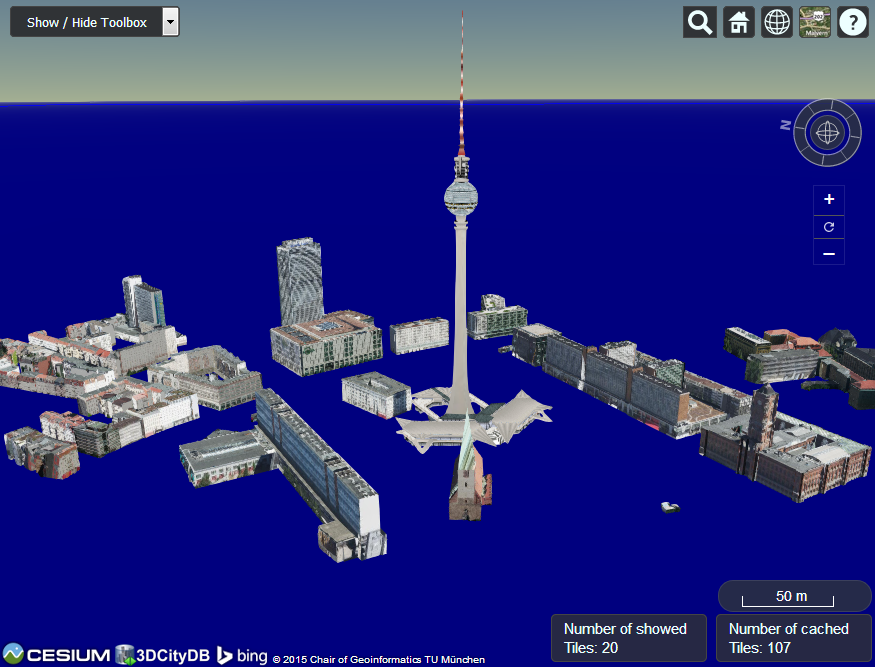
\includegraphics[width=\textwidth,height=\textheight,keepaspectratio]{3dcitydb.png}
  		\caption{Ukázka běhu aplikace 3DCityDB, model města Berlín}
  		\label{fig:3DcityDB}
	\end{figure}
        
        \subsubsection{Rozdíly ve funkcionalitě}
        
        Tato aplikace má sice blízko k~projektu Virtuální průvodce, ovšem zaměřuje se hlavně na celkové vizualizace měst, zejména pro potřeby městské správy, rozvoje infrastruktury apod. Tato bakalářská práce se naproti tomu bude zabývat zobrazením pouze menšího záběru z~velké databáze, díky čemuž by mělo být možné použít modely s~vyšším LOD. Zároveň si také tato práce klade za cíl větší obecnost (budeme pracovat s~klasickými 3D formáty, jako je .obj a ne specifickými geografickými formáty typu GML) a vyšší uživatelskou přívětivost.

    \subsection{Virtuální stará Praha}
    
    Projekt Virtuální Stará Praha vznikl v~roce 1999 pod vedením profesora J. Žáry jakožto spolupráce matematicko-fyzikální fakulty Univerzity Karlovy a katedry počítačové grafiky na FEL, ČVUT. Jedná se o~jednoduchou vizualizaci scény v~nejbližším okolí pražského Malostranského náměstí. \cite{VSP}
    
        \subsubsection{Softwarové požadavky}
        
        Aplikace je určená pro webové prohlížeče, je ovšem potřeba nainstalovat plugin VRML (Virtual Reality Modeling Language, jazyk pro modelování VR) prohlížeč, například Cortona VRML nebo též Cosmo Player VRML. Mezi další technické požadavky patří inernetový prohlížeč s~funkčním JavaScriptem a Java Applets. \cite{VSP}
        
        \subsubsection{Vlastnosti}
        
        Projekt VSP nabízí možnost procházení městské scény, která se dynamicky přizpůsobuje pozici uživatele. Z~tohoto důvodu je načítání jednotlivých modelů prováděno v~několika fázích podle sektoru, ve kterém se uživatel nachází. Tyto sektory se stále znovu vyhodnocují při pohybu městěm pomocí algoritmu, který nad sektory provádí množinové operace a podle toho zobrazuje modely. Nejvzdálenější budovy tedy nebudou načteny vůbec, bližší jsou vyobrazeny pouze tvarově bez textur (viz obr. \ref{fig:vsp2})  a teprve ty nejbližší budovy jsou načteny úplně (obr. \ref{fig:vsp1}).  \cite{VSP}
        
                
        
	
	\begin{figure}
  		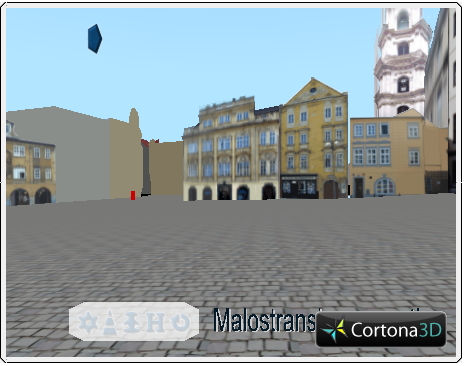
\includegraphics{vsp2.png}
  		\caption{Virtuální stará Praha, na levé části jsou vidět modely bez textur}
  		\label{fig:vsp2}
	\end{figure}
	
	
	\begin{figure}
  		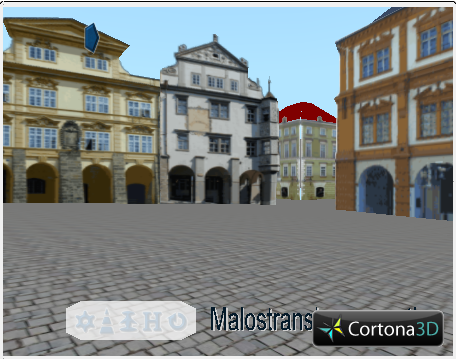
\includegraphics{vsp.png}
  		\caption{Ukázka běhu aplikace Virtuální stará Praha}
  		\label{fig:vsp1}
	\end{figure}

        \subsubsection{Rozdíly ve funkcionalitě}
        
        Oproti tomu tato bakalářská práce nebude pracovat s~dynamickým načítáním scény vyvolaným pohybem uživatele. Díky svému zaměření na VR není nutné importovat z~databáze víc domů, než těch v~bezprostředním okolí uživatele, neboť dále technologie VR uživateli nedovolí dojít. Bude sice možné provést posun do jiného sektoru města, ovšem tím budou také opuštěny všechny dosud načtené modely a namísto toho se uživatel přenese do úplně nově vygenerované scény.


	
	\subsection{Etruské hrobky}
	
	Tématikou vizualizace se taktéž zaobírají archeologové. Možnosti virtuální reality jim umožňují rekonstruovat velká archeologická naleziště a následně je zblízka procházet. Takto byly například zmapovány v~roce 2016 etruské hrobky Bartoccini a Bettini. Hrobky byly naskenovány a tím byly získány jejich 3D modely. 

        \subsubsection{Vlastnosti}	
	
	Naskenované modely měly ovšem příliš velké množství polygonů na to, aby bylo možné s~nimi efektivně pracovat, a proto byly v~programu 3Ds Max následně zjednodušeny. Dále jim byly přiděleny textury a byly naimportovány do Unity. Zde byla pak vytvořená jednoduchá VR aplikace pro jejich vizualizaci, která byla ovládána pomocí technologií Oculus a Kinect. Také zde byla implementována interaktivní místa, která uživateli zobrazila malé okno s~několika zajímavostmi (viz obr. \ref{fig:tomb} ). \cite{tombs}
	
	\begin{sidewaysfigure}
  		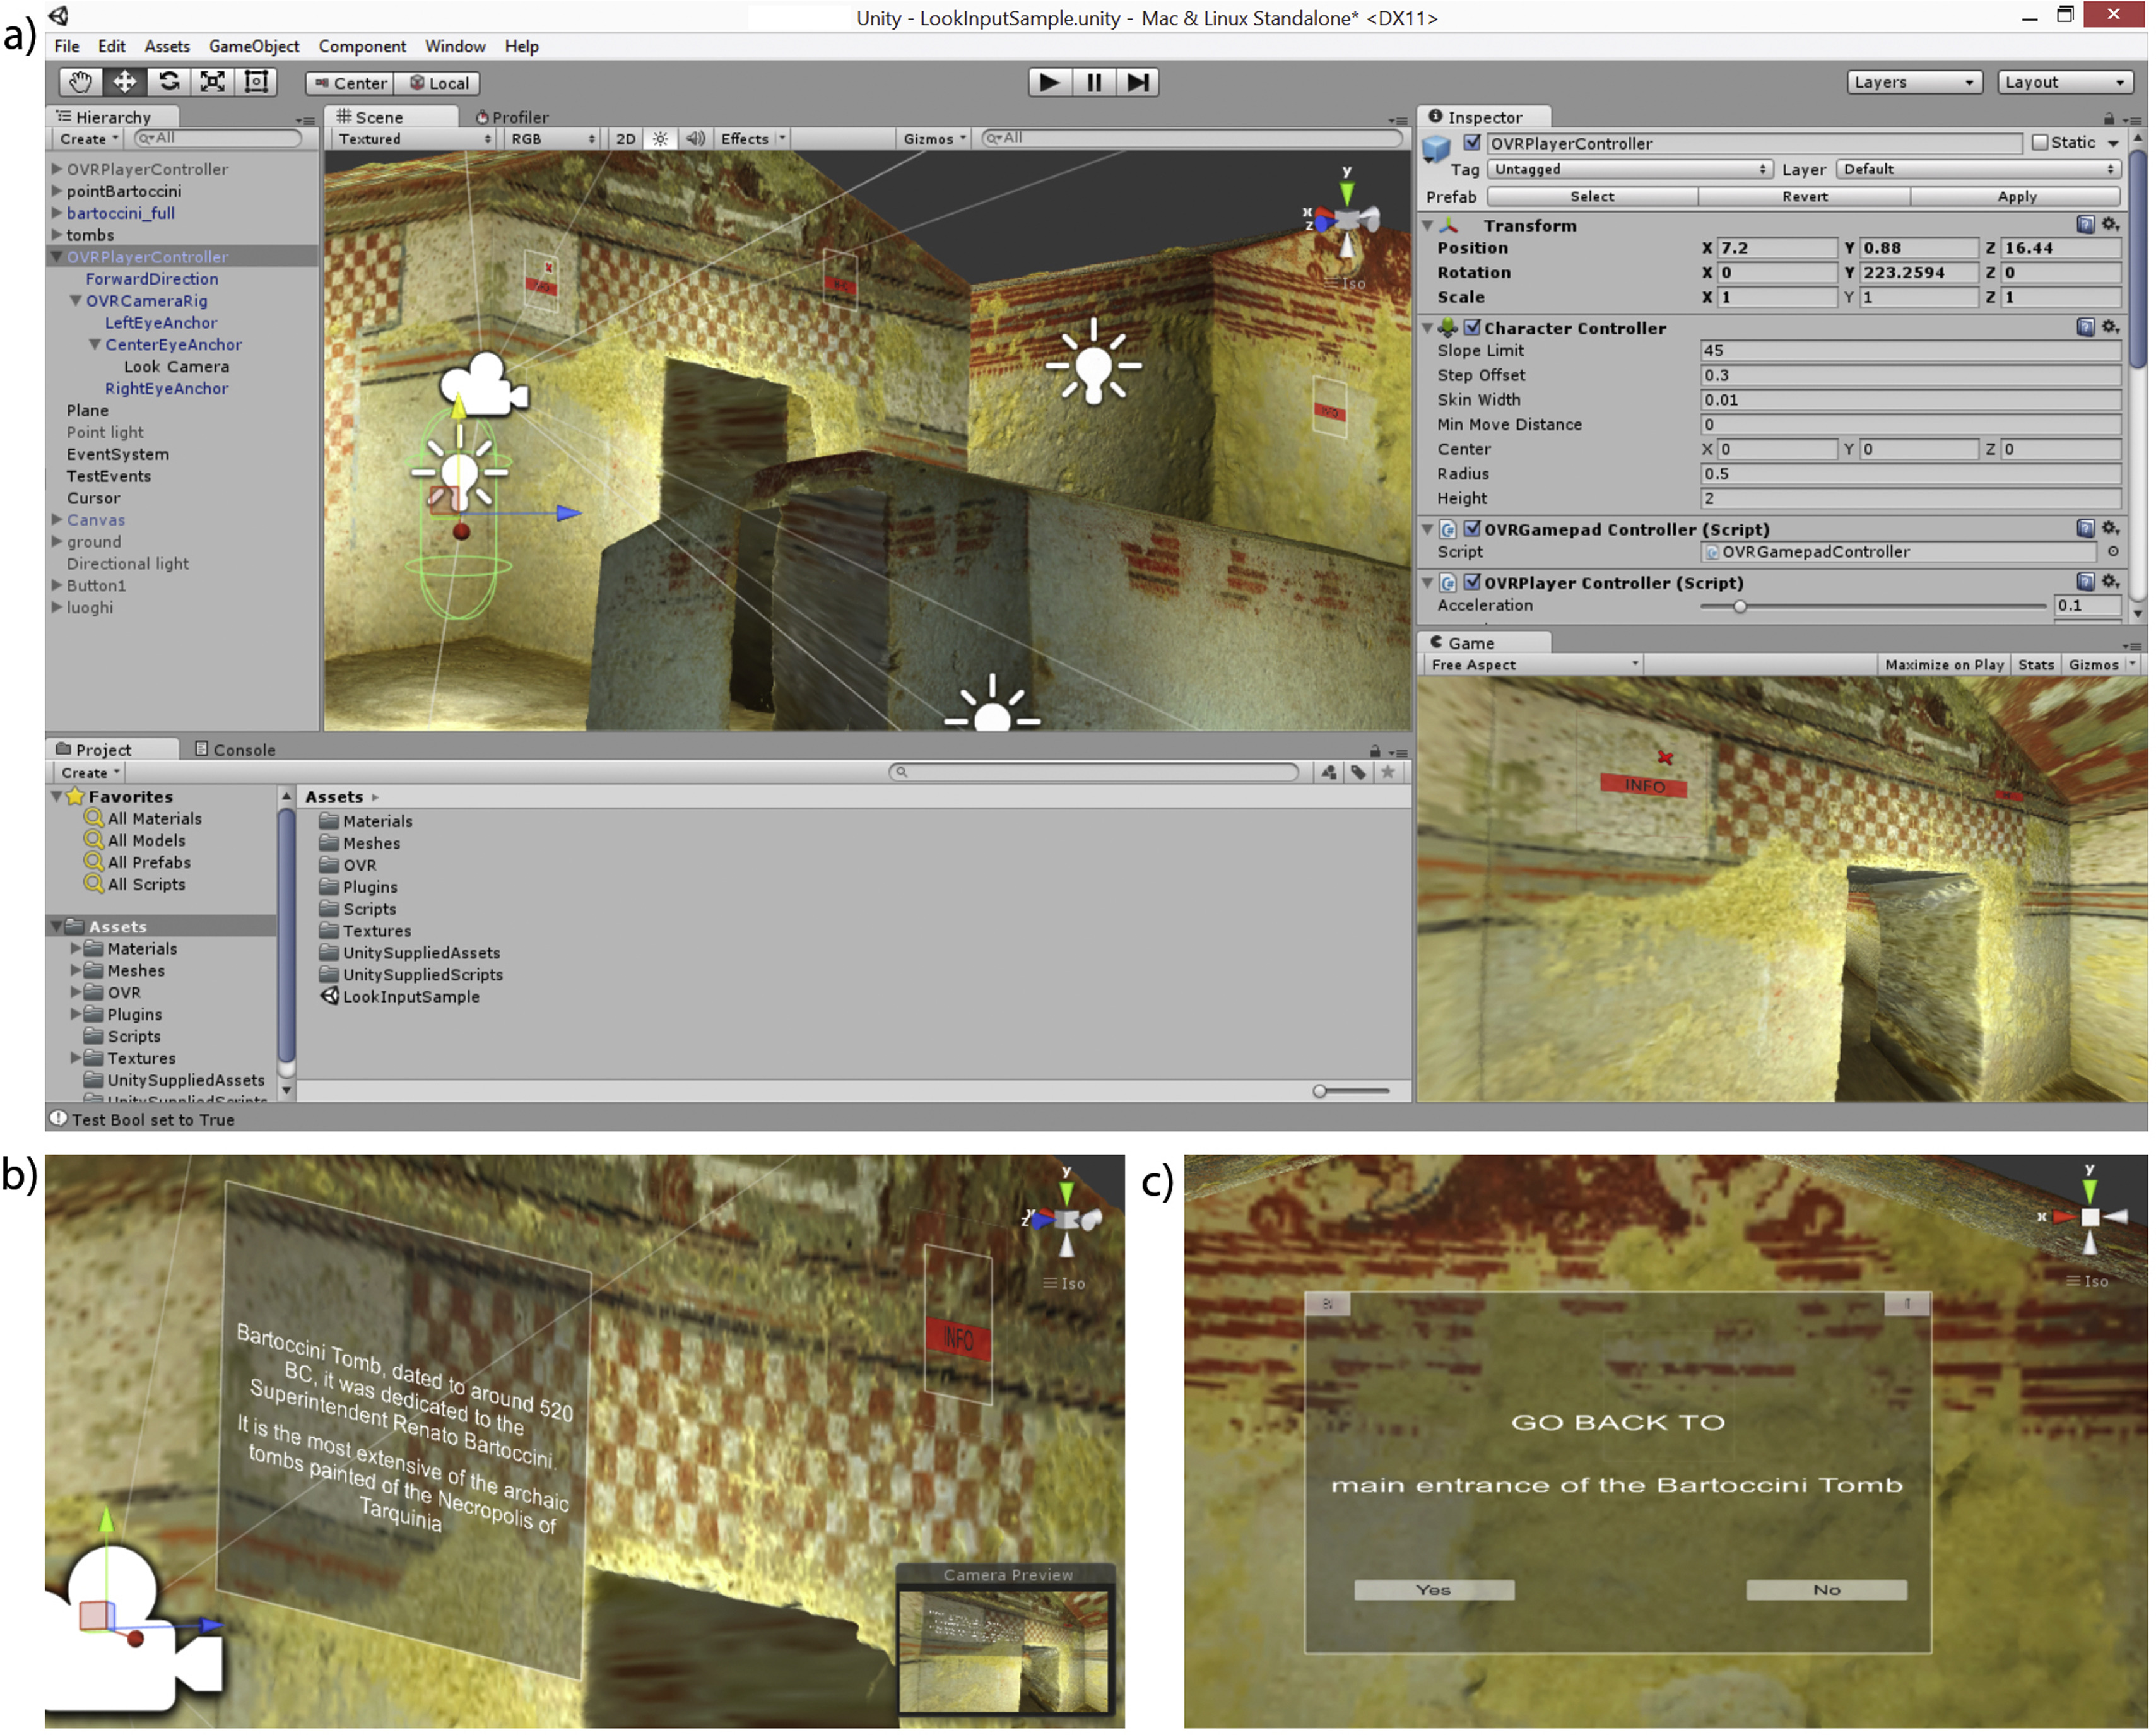
\includegraphics{tomb.jpg}
  		\caption{Aplikace vizualizující archelogické naleziště etruské hrobky v~Unity 3D \cite{tombs}}
  		\label{fig:tomb}
	\end{sidewaysfigure}

        \subsubsection{Rozdíly ve funkcionalitě}
Od této bakalářské práce se tento typ vizualizací liší hlavně použitím jednoho jediného statického modelu (hrobky, archeologického naleziště apod.). Aplikace Virtuální historický průvodce bude naproti tomu zobrazovat mnoho modelů, které bude dynamicky získávat z~databáze.

\subsection{Shrnutí}
 Všechny výše zmíněné aplikace mají blízko k~tématu této bakalářské práce, každý z~nich se ovšem trochu odlišuje funkcionalitou a hlavně cílovou skupinou.
 
  Z~hlediska cílové skupiny je této práci nejbližší projekt vizualizace etruských hrobek, protože se taktéž jedná o~aplikaci, která je určena jednak široké veřejnosti za účelem ponaučení a objevování starých světů, jednak odborníkům v~oblasti historie, kterým zjednodušuje bádání. Proto se od tohoto projektu tato bakalářská práce inspiruje v~možnosti interakce s~okolím a zobrazování modálních oken s~různými zajímavostmi o~daném objektu.

 Projekty 3DCityDB a Virtuální Stará Praha mají blíže k~této bakalářské práci tématikou, ovšem jsou zaměřeny na jiné cílové skupiny. 3DCityDB slouží hlavně městům jako takovým, naproti Virtuální Stará Praha je vizualizace pro každého. Problematické je zde u~obou těchto projektů ovšem ovládání a přístupnost. Oba tyto projekty vyžadují dosti složité nastavení webového prohlížeče, což může pro určité uživatele představovat jistou překážku. Navíc pak ani po úspěšném spuštění ani jedné z~těchto aplikací není úplně intuitivní jejich ovládání. 
 
 Analýza těchto řešení tak vnáší nejen vhled do funkcionality podobných aplikací, ale taktéž ukazuje, že při návrhu uživatelského rozhraní je u~podobných aplikací nutné vydat se jiným směrem. V~kapitole \ref{sec:GUI} bude blíže rozebráno zvolené řešení návrhu uživatelského rozhraní, které se bude snažit být uživatelsky přijatelnější a co nejvíce intuitivní.
	
	\section{Analýza použitých technologií}
	
	V~této sekci budou rozebrány jednotlivé technologie, které byly zvoleny pro implementaci projektu Virtuální historický průvodce.

		\subsection{Unity}	
		
		Unity 3D je robustní software, který slouží především k~vývoji počítačových her. Nabízí široké využití jak pro programátory, tak pro grafiky nebo i game designéry. Orientuje se převážně na 3D aplikace (odtud název), ovšem umožňuje i vývoj ve 2D. V~dnešní době patří mezi nejzákladnější výbavu vývojářů aplikací pro VR.
		
		\subsubsection{XR v~Unity}
		
		Unity podporuje všechny technologie sdružené s~VR, které se souhrnně označují \uv{XR}. Řadíme sem jednak klasické VR technologie, jednak technologie rozšířené reality (augmented reality - AR) či smíšené reality (mixed reality - MR). Mezi konkrétní technologie, které je možné sem zařadit, jmenujme například Oculus, HTC VIVE, Microsoft Hololens, Playstation VR, Cardboard a další.\cite{UnityVR}
		
		\subsubsection{Nastavení podpory pro VR v~Unity}
		
		Aplikace v~Unity může být v~nastavení upravena pro VR mód. Pokud je v~Player settings povolena podpora VR, je možné nastavit seznam všech technologií, které bude aplikace podporovat v~tom pořadí, jak jsou v~tomto seznamu uvedeny. Toto se dá nastavit jednak v~GUI (grafickém uživatelské rozhraní) Unity, jednak v~kódu pomocí proměnných XRSettings.supporteddevices. Není možné přidávat nová zařízení dynamicky, seznam technologií musí být úplný již při kompilaci aplikace.

Tímto nastavením se změní pozice kamery tak, aby podporovala HMD (head mounted display, neboli VR brýle), což mimo jiné zajistí, že pohledová matice a matice projekce se přizpůsobí pohybům hlavy. Všechny potřebné informace o~pozici hlavy se zajistí ještě před samotným renderováním obrazu, což zabrání různým negativním vedlejším efektům, mezi které patří například nevolnost či ztráta rovnováhy.

Vývojáři jednotlivých VR technologií vytvořili pro uživatele Unity speciální balíčky, které je možno stáhnout zdarma v~Unity Asset store. Tyto balíčky obsahují nastavení pro vývoj ve VR.\cite{UnityVR}

		\subsection{Virtual Reality Toolkit}
		
		VRTK neboli Virtual Reality Toolkit je sada skriptů, které usnadňují vývoj aplikací pro VR v~Unity 3D. VRTK momentálně plně podporuje technologie SteamVR a Oculus, do budoucna bude zavádět i podporu technologií Daydream a XimmerseVR. Mezi jeden z~nejpraktičnějších aspektů jejich využití patří testování VR módu aplikace bez nutnosti zapojení VR headsetu díky vestavěnému VR simulátoru. VRTK je uvedeno na trh pod licensí MIT \cite{VRTKlic}, která umožňuje volné šíření i modifikaci tohoto systému.
		
\subsubsection{Simulátor VRTK}
VRTK SDKManager je sada skriptů, která obsahuje základní ovládací prvky pro simulátor VR v~Unity. Jedná se o~přenositelný samostatný balíček, který je možno importovat z~Unity Asset Store do jakéhokoli projektu v~Unity. Tím získáme balíček VRTK, ve kterém jsou předpřipravené ukázkové scény se simulátorem. Objekt simulátoru zvaný VRTK můžeme z~těchto scén překopírovat do vlastních scén, je ovšem nutné vymazat nyní již nadbytečnou hlavní kameru. Vestavěné uživatelské rozhraní SDKManageru umožňuje přepínat libovolně mezi ovládáním přes simulátor a ovládáním přes nastavené VR zařízení. \cite{VRTK} Toto nastavení je vidět na obrázku \ref{fig:VRTKsetup}.

\subsubsection{Ovladače pohybu}
Velká výhoda VRTK je v~tom, že nabízí předpřipravené objekty LeftController a RightController, které zaznamenávají pohyby rukou. Je tedy jedno, zda bude výsledná aplikace ovládána tím nebo oním VR zařízením, nebo zda jenom simulátorem, všechny události vyvolané pohybem jsou zpracovávány stejně. K~tomuto účelu nabízí VRTK rozhraní VRTK\_ControllerEvents, které obsluhuje všechny události vyvolané uživatelem a dovolí programátorovi vytvořit pro ně specifické handlery.

\subsubsection{VR ukazatel}
Pro interakce s~okolím za pomocí takzvaného pointeru, neboli ukazatele v~podobě barevného laseru, který umožňuje interakci s~objekty na dálku, má VRTK taktéž vestavěné funkce. Stačí k~ovladačům pohybu připojit knihovní skripty VRTK\_Pointer (pro základní funkcionalitu ukazatele), VRTK\_Straight Pointer Renderer (pro zobrazení ukazatele za pomocí barevných čar) a ideálně taktéž VRTK\_UI Pointer (pro interakci s~uživatelským rozhraním).



	\begin{figure}
  		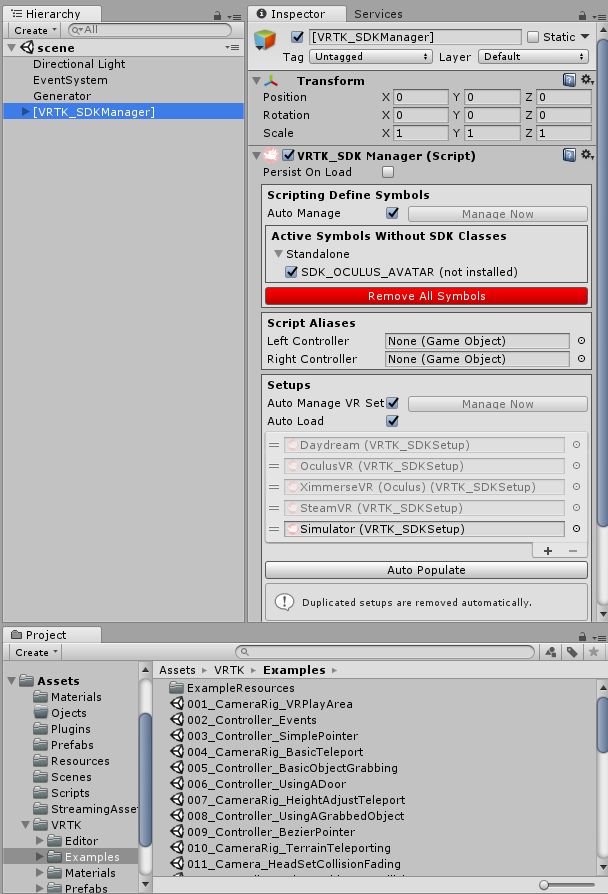
\includegraphics{VRTKsetup.png}
  		\caption{Nastavení VRTK}
  		\label{fig:VRTKsetup}
	\end{figure}
	
	\subsection{C\#, .NET, MONO}
	
	Unity 3D umožňuje vývojářům na výběr ze dvou programovacích jazyků: JavaScript a C\#. Protože C\# je v~Unity už více zavedený (a tedy nabízí větší množství zdrojů a návodů spojených s~Unity), je i kód této bakalářské práce sepsán v~C\#. Unity ovšem nepoužívá základní C\# framework .NET, nýbrž jeho open source verzi Mono. Níže jsou blíže rozepsané vlastností a odlišnosti těchto technologií.
	
	\subsubsection{C\#}
	C\# je objektově orientovaný programovací jazyk vyvíjený firmou Microsoft. Podobně jako Java nepředává své instrukce přímo hardwaru, ale stojí za ním virtuální stroj, tzv. CLR (Common Language Runtime). Jedná se o~jazyk velice blízký jak jazyku C++, tak jazyku Java.
	
	
	\subsubsection{.NET Framework}
	Jedná se o~framework, který velice úzce navazuje na výše zmíněný jazyk C\#. Jazyk C\# je s~.NETem tak úzce provázaný, že je takřka nemožné jej používat samostatně bez volání alespoň některých knihovních funkcí z~.NETu. .NET bohužel není multiplatformní, je spustitelný pouze pod MS Windows.
	
	\subsubsection{Mono}
Mono je open source verze .NET frameworku. Jedná se o~nástroj, který umožňuje vývoj aplikací ve stylu C\# a .NET i pro jiné platformy, než je MS Windows. Aplikace vyvíjené v~Mono jsou plně přenositelné jak na Linux, Mac, Windows, tak i na mnoho dalších platforem. Mono v~sobě spojuje následující komponenty:
	
	\begin{itemize}
	\item C\# kompilátor
	\item Mono Runtime
	\item .NET knihovna tříd
	\item Mono knihovna tříd \cite{mono}
	\end{itemize}
	
	
    \subsection{Swagger}
    
    Pro návrh API byla zvolena technologie Swagger, která umožňuje vazby zaznamenat ve formátu YAML (formát pro serializaci strukturovaných dat) a JSON (JavaScriptový objektový zápis).
    
    Technologie Swagger umožňuje rychlý vývoj REST API. Řídí se primárně heslem \uv{neprve návrh, kód až poté}. Jedná se tedy o~několik technologií (Swagger Editor, Swagger UI a Swagger Codegen) umožňující vývoj prezentační vrstvy aplikací bez nutnosti mít již plně naimplementovanou business vrstvu. Naopak, business vrstva může být vygenerována ze samotného návrhu rozhraní. K~tomuto účelu slouží konkrétně Swagger Codegen, který podle nadefinovaného API dokáže vygenerovat kódy pro server, které jsou potřeba. \cite{swagger}
	
	
	
			

	
\chapter{Návrh}
	\section{Návrh architektury}
	Architektura celého projektu je navržena jako třívrstvá (viz obrázek \ref{fig:architektura}). Tato bakalářská práce se zabývá návrhem a implementací dvou svrchních vrstev, tedy prezentační a business vrstvy. Funkcionalita jednotlivých vrstev je popsána níže podrobněji.
	
	
	\begin{figure}
  		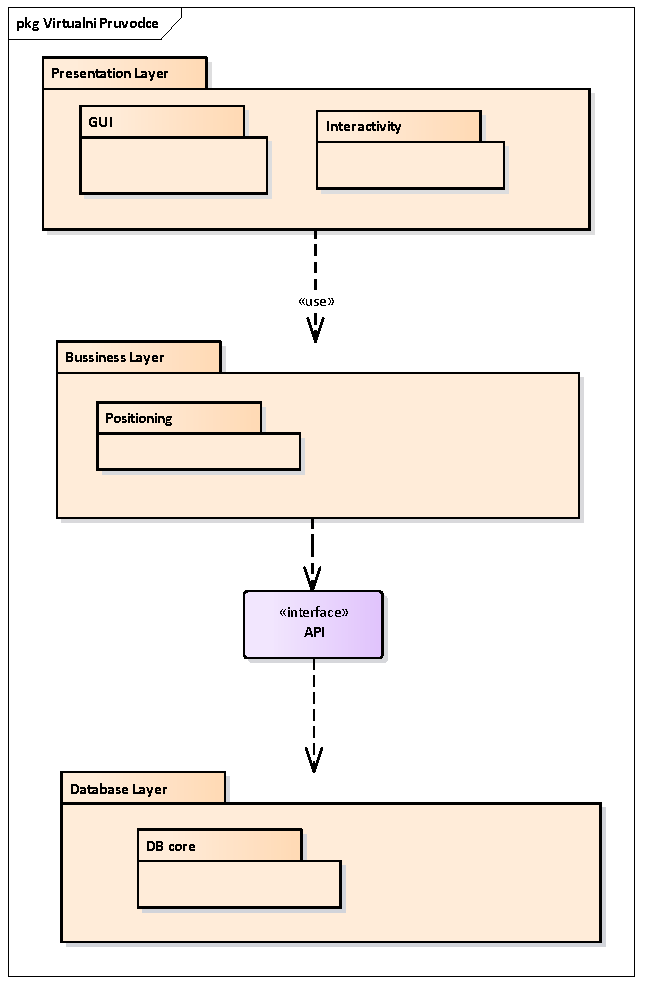
\includegraphics[width=\textwidth,height=\textheight,keepaspectratio]{appArch.pdf}
  		\caption{Návrh architektury celé aplikace}
  		\label{fig:architektura}
	\end{figure}
	
	\subsection{Prezentační vrstva}
	Prezentační vrstva zajišťuje zobrazení celé scény a veškerou komunikaci přímo s~uživatelem. Je implementována v~souboru Generator.cs a dalších. Konkrétně se jedná o:
		\begin{itemize}
			\item Vykreslení jednotlivých modelů
			\item Zobrazení GUI
			\item Interaktivní prvky
		\end{itemize}

	\subsection{Business vrstva}	
	 Naproti tomu business vrstva se zabývá logickým vyhodnocením dat získaných z~datové vrstvy. Sem mimo jiné spadá:
	 \begin{itemize}
			\item Logika rozmisťování modelů
			\item Vyhodnocování dotazů zadaných uživatelem
			\item Nasvětlení scény
			\item Přiřazení textur načteným modelům			
		\end{itemize}
	 
	 \subsection{Datová vrstva}
Nejspodnější datová vrstva (data layer DL) obsahuje datové úložiště, které bude v~PostgreSQL databázi obsahovat všechny modely, textury, jejich jednotlivé verze atd. Jedná se o~robustní databázi, která bude zpracována nezávisle na ostatních vrstvách. Tato datová vrstva bude jádrem celého projektu, který bude kromě modulu VR (zpracovávaného v~této práci) přenositelný na mnohá další zařízení. Proto je databázová vrstva zpracovávána nezávisle v~rámci jiné bakalářské práce (její datový model viz obr. \ref{fig:ERmodel} ). Tudíž bylo pro komunikaci s~ní navrženo API. Jeho podrobná specifikace je uvedena v~sekci \ref{sec:API}.
	
	\begin{sidewaysfigure}
  		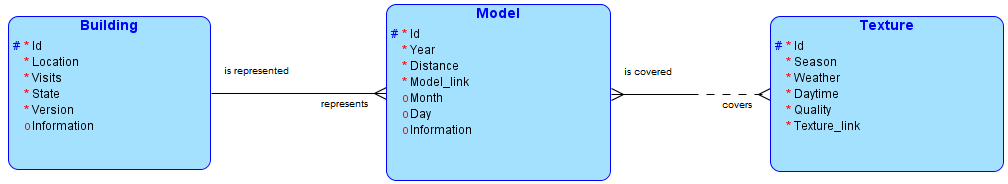
\includegraphics[width=\textwidth,height=\textheight,keepaspectratio]{ERmodel.png}
  		\caption{ER (entitně vztahový) model databáze \cite{cernyVit}}
  		\label{fig:ERmodel}
	\end{sidewaysfigure}
	
		\section{Funkční a nefunkční požadavky}
	Tato kapitola se zabývá rozborem funkčních a nefunkčních požadavků, které bude výsledná aplikace podporovat či nikoliv. Tyto požadavky pomáhají vymezit rámec aplikace a její celkovou finální podobu.
	
	\subsection{Funkční požadavky}	
	Tato sekce obsahuje popis funkčních požadavků, které jsou na systém kladeny.
	
	\begin{description}
	
 		\item \textbf{F1 - vizualizace městské scény}
 		 			
 			Systém přenese uživatele na konkrétní místo ve městě, jinými slovy vygeneruje modely v~nejbližší blízkosti podle konkrétní specifikace požadované uživatelem. Zohlední také světelné a atmosférické podmínky, podle konfigurace scénu tedy zobrazí například ve tmě, ráno, v~dešti, za sněhu apod. K~tomuto bude potřeba načíst modely z~databáze, rozmístit je v~dané konfiguraci, nastavit textury a materiály podle počasí a přidat skybox.

 		\item \textbf{F1.1 - interaktivita}
 		
 		Systém umožní uživateli se svým okolím interagovat, a tím je lépe prozkoumávat. Například při ukázání na dům se zobrazí jednoduché informace o~tomto domě, dále by bylo například možné zhasnout či rozsvítit lampu a tím změnit nasvícení modelů atd.
 		
 		\item \textbf{F3 - modul pro VR}
 		
 		Během vývoje bude aplikace vytvářena pro PC, celkový výsledek bude ovšem funkční pro technologii VR brýlí. Jelikož Unity3D engine podporuje široké množství VR technologií, bude výsledná aplikace přenositelná na téměř jakékoli technologie virtuální reality. Protože základní myšlenka aplikace je vizualizace města pouze v~nejbližším okruhu uživatele, skvěle tak koresponduje s~omezeným prostorem, které technologie VR v~dnešní době podporují.
 		
 		\item \textbf{F4 - administrační interface}
 		
 		Aplikace bude uživatelům také umožňovat vlastní konfiguraci. Systém bude možné přenastavit dle vlastních preferencí, bude tedy možné nahrát do města nové domy, nově je rozmístit a vložit je do databáze. Tato funkcionalita je určena pouze pro specifické uživatele, proto bude tato umístěna stranou ve vedlejším menu.
 	\end{description}	
 		
\subsection{Nefunkční požadavky}	
	Tato sekce obsahuje popis nefunkčních požadavků, které nesouvisejí přímo s~funkčností systému, ale přesto jsou pro správný provoz systému důležité.
			
 		\begin{description}
 		
 		\item \textbf{N1 - komunikace s~datovým úložištěm}
 		
 		Aplikace bude modely získávat z~vnější databáze, ke které bude přistupovat pomocí REST API. Tento přístup by měl zajistit efektivní zobrazování scény v~závislosti na konkrétní lokaci, kdy se zobrazí pouze ty modely, které jsou v~nejbližší blízkosti daných souřadnic. V~databázi budou mimo samotných modelů uloženy také jejich transformační matice pro správné umístění v~prostoru a textury pro různá počasí.
 		
 		\item \textbf{N2 - simulátor pro desktop PC}
 		
 		Systém bude mít pro potřeby testování i vestavěný simulátor, který bude napodobovat ovládání přes VR konzoli. Díky tomu nebude nutné k~vývoji ani k~prvotnímu testování vlastnit VR headset.
 		
 		
 	\end{description}	
 	
	\section{Případy užití}
	Tato kapitola se zabývá rozborem aplikace z~pohledu uživatele. Přehled případů užití níže a obrázek \ref{fig:UCdiagram} zachycují všechny základní scénáře, které při používání aplikace mohou nastat.
	
	\begin{description}
	
 		\item \textbf{UC1 - Procházení města ve VR}
 		
 			Systém umístí uživatele na požadovanou pozici ve městě.
 		 	
 		 	\begin{enumerate}
 		 		\item Případ užití začíná ve chvíli, kdy si uživatel nasadí VR headset a objeví se na připravené startovní pozici.
				\item Systém uživateli po stisknutí tlačítka menu nabídne dialog, který umožní uživateli přesun na jinou lokalitu.
				\item Uživatel zvolí ulici, denní dobu, počasí a roční období, ve kterém se chce ocitnout (výchozí nastavení je léto, odpoledne, slunečno).
				\item Systém uživatele \uv{přenese} na danou lokalitu tím, že kolem něj vygeneruje potřebné 3D modely domů ve správné konfiguraci (pozice, natočení, textury, skybox)
				\item Uživatel může v~omezeném prostoru definovaném VR headsetem procházet své okolí.
			\end{enumerate} 		 			
 			

 		\item \textbf{UC2 - Interakce s~městem}
		Basic Path: Uživatel při procházení města interaguje s~budovami. 		
 		
 		\begin{enumerate}
				\item Uživatel klikne (v~PC verzi) či gestem ukáže (ve VR verzi) na konkrétní budovu.
				\item Systém zobrazí okénko s~několika informacemi o~daném objektu, jmenovitě název, účel, datace, zajímavosti (např. Faustův dům, 1378, popis legendy o~Faustovi, dnes součástí Všeobecné fakultní nemocnice).
 		\end{enumerate}
 		
 		Alternate Path: Uživatel interaguje s~jednotlivými objekty.
 		\begin{enumerate}
				\item Uživatel zjistí, že je možné interagovat s~objektem díky upozornění.
				\item Uživatel klikne (v~PC verzi) či gestem ukáže (ve VR verzi) na konkrétní objekt.
				\item Systém změní nějaké vlastnosti objektu, například zhasne lampu apod.
 		\end{enumerate}
 		
 		\item \textbf{UC3 - Úprava města}
 		
 		Pokročilý uživatel využívá administrátorské funkce.
 		\begin{enumerate}
    		\item Uživatel poklepá na ikonu vedlejšího menu v~pravém honím rohu a zvolí položku \uv{Architect mode}.
    		\item Systém uživateli zobrazí město z~ptačí perspektivy a zobrazí administrátorské menu.
    		\item Uživatel v~administrátorském menu vybere položku \uv{vložit budovu}.
    		\item Systém uživateli zobrazí okno s~pohledem do systému souborů, kde si uživatel může najít soubor 3D modelu nově vkládané budovy.
    		\item Uživatel pomocí myši umístí budovu na požadované místo.
    		\item Systém otevře potvrzovací okno, zda si je uživatel jistý pozicí nové budovy.
    		\item Uživatel potvrdí své rozhodnutí.
    		\item Systém uloží budovu do databáze.
 		\end{enumerate}
		
 		
 	\end{description}	
 	
 	\begin{figure}
  		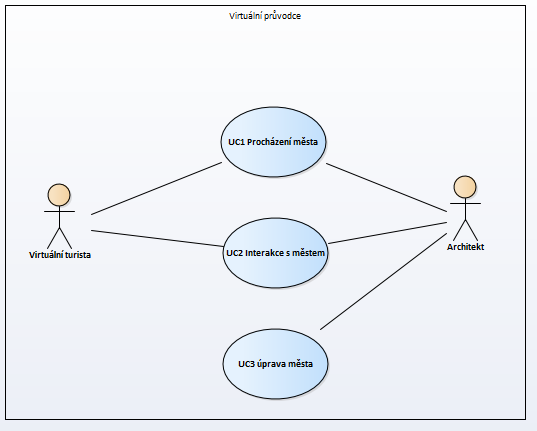
\includegraphics{UCdiagram.png}
  		\caption{Diagram případů užití}
  		\label{fig:UCdiagram}
	\end{figure}
	
	\section{Návrh použitého API}
	\label{sec:API}
    
    Jelikož na projektu Virtuální Průvodce bude spolupracovat více lidí, je potřeba navrhnout API pro vzájemnou komunikaci jednotlivých části aplikace. Konkrétně se jedná o~propojení databáze 3D modelů se samotným zobrazovacím modulem.

    
      \subsection{Položky API}
      
      API bylo navrženo co nejjednodušeji, ale zároveň tak, aby  podporovalo všechny požadavky, které nad databázi mohou být vzneseny. Databáze tedy vrátí na konkrétní dotaz nad touto množinou specifickou odpověď, s~pomocí které bude model umístěn do scény v~potřebné konfiguraci. Podrobné specifikace parametrů jsou popsány níže, jejich návrh v YAMLu je vidět na obr \ref{fig:yamlAPI}.
	
	\begin{description}
		\item[Název modelu]
			Jedná se o~popis modelu, který pomáhá k~jeho identifikaci. Oproti ID slouží spíše ke zpřehlednění, případně jakožto nadpis k~dodatečným informacím o~modelu.

		\item[Informace o~modelu]
			Stručný popis konkrétní stavby, který bude možno ve finální aplikace zobrazit při interakci s~daným modelem.

		\item[ID modelu]
			Jednoznačné ID sloužící k~jeho identifikaci v~databázi.

		\item[Souřadnice]
			Tento parametr bude rozdělen na 3 podsložky, a to na rotaci, zvětšení (scale) a pozici (transpozici). Toto zjednoduší dotazování nad databází, například pro zobrazování všech modelů v~určité vzdálenosti bude potřeba pouze hodnota parametru určující pozici.
			
		\item[Roční období]
			Čtyři klasické roční období uložené pomocí typu enum.

		\item[Link na texturu]
			Odkaz do FS (systému souborů) na bitmapu dané textury.

		\item[Link na 3D model]
			Odkaz do FS na link 3D modelu v~daném formátu (např. obj).

		\item[Samotný 3D model]
			Do budoucna budeme experimentovat i s~možností uchovávání samotného 3D souboru v~databázi namísto pouze informaci o~jejím umístění na FS.
			
		\item[Počasí]
			Rozlišujeme jen několik základních typů počasí (pomocí enum) a to:

	    	\begin{itemize}
    			\item slunečno (sunny)
    			\item deštivo (rainy)
    			\item zataženo (cloudy)
    			\item sníh (snow)
    		\end{itemize}

		\item[Denní doba]
			Taktéž charakterizována jednotlivými typy za pomoci datového typu enum:
	    	\begin{itemize}
    			\item ráno
    			\item odpoledne
    			\item večer
    			\item noc
    		\end{itemize}
			
	\end{description}
	
	\begin{figure}
  		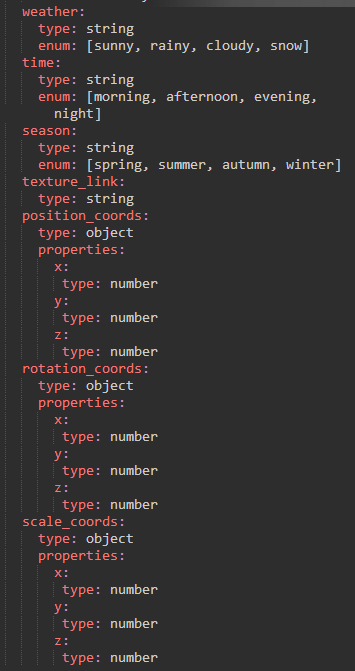
\includegraphics{api.png}
  		\caption{API v~YAML}
  		\label{fig:yamlAPI}
	\end{figure}
	
\chapter{Implementace}

	\section{Napojení na datové úložiště}
		    Tato kapitola se zabývá způsobem propojení aplikace Virtuální průvodce s~externím datovým úložištěm. V~první části je zmíněna varianta přímého napojení na databázi, která sice není použita ve výsledné aplikaci, ovšem kvůli jednoduššímu přístupu k~datům sloužila jako prvotní prototyp celé aplikace. Pro finální produkt je toto řešení ovšem nevhodné, kvůli velkému rozsahu celého projektu bude použito REST API. Popis komunikace přes toto API s~pomocí souborů JSON je popsán v~dalších částech této sekce.
    

\subsubsection{Přímé propojení s~databází}
 Toto téma bylo hlavní náplní týmového projektu HK (Hradec Králové) v~rámci předmětu SP2 (Softwarový týmový projekt 2). Kromě autorky této bakalářské práce se na dané semestrální práci podíleli také studenti FITu Josef Struž a Iuliia Ostrokomorets. 
   
    K~tomuto účelu byla použita knihovna NpSQL. V~souboru Sqlconnector.cs ve třídě Sqlconnector je uložená proměnná \uv{connecting}, která v~sobě obsahuje informace o~připojení k~databázi (Server, Port atd.). Při inicializaci této třídy se vytvoří propojení s~databází. Tato třída v~sobě uchovává list Modelů (\uv{Model} je struktura, která obsahuje všechny informace o~daném modelu, které byly získány z~databáze). Nejdůležitější části tohoto kódu jsou níže:
    \begin{lstlisting}[frame=single]
    public Sqlconnector()
    {
        connection = new NpgsqlConnection(connstring);
        connection.Open();
        listItems();              
    }

    void listItems()
    {
        NpgsqlCommand command = new NpgsqlCommand("SELECT * FROM models", connection);
        NpgsqlDataReader dataReader = command.ExecuteReader();
        
    }
	\end{lstlisting}
    
    \subsubsection{JSON v~Unity}
	
	Finální aplikace ovšem nekomunikuje s~databází přímo, jako to bylo implementováno v~projektu pro předmět SP2, nýbrž přes REST API (viz návrh použitého API v~kapitole \ref{sec:API}). Navržené API bude komunikovat s~databázovým serverem za pomoci souboru JSON. Ukázková odpověď serveru v podobě souboru JSON používaná při testování tohoto projektu je k vidění níže.
	\begin{lstlisting}[frame=single]
	{
    "model_name": "house42",
    "model_ID": 6,
    "info": "some random info",
    "file_link": ".\\MedHouse\\housemedieval.obj",
    "file": "void",
    "weather": "sunny",
    "time": "afternoon",
    "season": "spring",
    "texture_link": ".\\MedHouse\\HouseMed_Diff.jpg",
    "position_coords": {
      "x": -35,
      "y": 13.5,
      "z": 10
    },
    "rotation_coords": {
      "x": 0,
      "y": 90,
      "z": 0
    },
    "scale_coords": {
      "x": 2,
      "y": 2,
      "z": 2
    }
  }

\end{lstlisting}
	
	 JSON je zavedený standard, takže jej Unity podporuje a nabízí i knihovny, které umožní jeho deserializaci. Jedná se konkrétně o~vestavěnou třídu JSONUtility, která nabízí rozhraní pro serializaci i deserializaci JSON souboru. Je tedy možné snadno namapovat obsah JSON souboru do vytvořené třády s~příslušnými třídními proměnnými, na které je možné JSON namapovat. \cite{UnityJSON}

V~tuto chvíli ovšem ještě není zavedena podpora polí objektů v~rámci jednoho JSONu. \cite{UnityJSON} Vzhledem k~tomu, že API pro projekt Virtuální Průvodce očekává JSON soubory právě v~tomto formátu, neboli pole modelů budov v~jediném souboru, je nutné tuto funkcionalitu dodatečně zajistit za pomoci dodatečných obalovacích tříd. Můžeme si tedy nadefinovat ještě jednou další třídu, která bude sloužit jako obal, který v~sobě bude uchovávat pole modelů. V~implementaci byla tato třída pojmenována Root, neboť je jakýmsi kořenem všech podtříd v~rámci JSON souboru. Toto pole modelů má ovšem název, který by nebylo možno na nic v~souboru JSON namapovat. To se dá jednoduše spravit tím, že před přijaté pole modelů od API po přečtení připojíme řetězec obsahující název proměnné, do které se uloží pole modelů s~pomocí následující funkce.

\begin{lstlisting}[frame=single]
public string fixJson(string value)
    {
        value = "{\"models\": [" + value + "] }";
        return value;
    }

\end{lstlisting}

Aby byla serializace možná, je nutné nad deklaraci mapovací třídy Model přidat Unity direktivu [System.Serialiazble]. Všechny definice tříd, na které se JSON namapuje, jsou k~vidění níže. 

\begin{lstlisting}[frame=single]
public class Root
{
    public Model[] models;
}


public class Coords 
{
    public float x;
    public float y;
    public float z;
}

[System.Serializable]
public class Model
{
    public string model_name;
    public int model_ID;
    public string info;
    public string file_link;
    public string file;
    public string weather;
    public string time;
    public string season;
    public string texture_link;
    public Coords position_coords;
    public Coords rotation_coords;
    public Coords scale_coords;
}
\end{lstlisting}

	\subsubsection{Mono a HTTPS}
	
	Výchozí nastavení Mono (na kterém C\# v~rámci Unity běží) je v~rámci bezpečnosti vysoce selektivní, slovy vývojářů \uv{Mono nevěří nikomu!} \cite{mono}. Pokud je tedy potřeba pomocí HTTPS protokolu přistupovat k~serveru, je pravděpodobné, že tomuto přístupu bude zamezeno. Řešení tohoto problému je funkce, která projde všechny chyby, které se v~žádosti o~certifikáty naskytly, a manuálně vytvoří nový certifikát X509, který znovu sama zkontroluje. Zavoláním této funkce těsně před přístupem k~API s~pomocí GET zajistí správný průběh komunikace mezi serverem a aplikací. Níže je ukázka funkce, kterou za tímto účelem nadefinovali uživatelé Unity \cite{unityFAQ}.
	
	\begin{lstlisting}[frame=single]
public bool MyRemoteCertificateValidationCallback(System.Object sender,
   X509Certificate certificate, X509Chain chain, SslPolicyErrors sslPolicyErrors)
    {
        bool isOk = true;
        // If there are errors in the certificate chain,
        // look at each error to determine the cause.
        if (sslPolicyErrors != SslPolicyErrors.None)
        {
            for (int i = 0; i < chain.ChainStatus.Length; i++)
            {
                if (chain.ChainStatus[i].Status == X509ChainStatusFlags.RevocationStatusUnknown)
                {
                    continue;
                }
                chain.ChainPolicy.RevocationFlag = X509RevocationFlag.EntireChain;
                chain.ChainPolicy.RevocationMode = X509RevocationMode.Online;
                chain.ChainPolicy.UrlRetrievalTimeout = new TimeSpan(0, 1, 0);
                chain.ChainPolicy.VerificationFlags = X509VerificationFlags.AllFlags;
                bool chainIsValid = chain.Build((X509Certificate2)certificate);
                if (!chainIsValid)
                {
                    isOk = false;
                    break;
                }
            }
        }
        return isOk;
}
	\end{lstlisting}
	
	\subsection{HTTP propojení s API}
	Následující kód provádí už samotný přístup k API přes HTTP (hyper text transfer protocol). Veškerá logika popisovaná v této sekci je uložena v prováděna třídou DataReader v souboru DataReader.cs.
	
	\begin{lstlisting}[frame=single]
	 private string GetJSONfromAPI()
    {
        HttpWebRequest request = (HttpWebRequest)WebRequest.Create(String.Format(uri));

        //a special function to add a certificate (otherwise Mono won't allow any connections]
        ServicePointManager.ServerCertificateValidationCallback = MyRemoteCertificateValidationCallback;

        HttpWebResponse response = (HttpWebResponse)request.GetResponse();
        StreamReader reader = new StreamReader(response.GetResponseStream());
        string jsonResponse = reader.ReadToEnd();
        Debug.Log("API response = " + jsonResponse);
        jsonResponse = fixJson(jsonResponse);
        Debug.Log("Fixed JSON = " + jsonResponse);
        return jsonResponse;
    }

    public void LoadGameData() {
        string jsonresponse;
        jsonresponse = GetJSONfromFS();

        root = JsonConvert.DeserializeObject<Root>(jsonresponse);       

    }
	\end{lstlisting}
	
	
	\section{Vykreslení v~Unity}
    Pro vykreslování se využívá GameObject Generator ze souboru Generator.cs. Generátor má v~sobě uložený vzor budovy \uv{Building}. Při spuštění se vytvoří nový GameObject \uv{Buildings}, který je rodičem všech ostatních budov (pokud by bylo potřeba smazat nebo měnit velikost aktuální scény, stačí upravit pouze tohoto rodiče) a také se vygenerují všechny budovy. Každá budova obsahuje funkci Set(Model), která načte mash (pomocí třídy FastObjImporter) a pomocí zobrazovací matice nastaví pozici, rotaci a velikost. Ukázka běhu aplikace s~načtenými modely je vidět na obrázku \ref{fig:buildings}
    
    

\begin{figure}
  		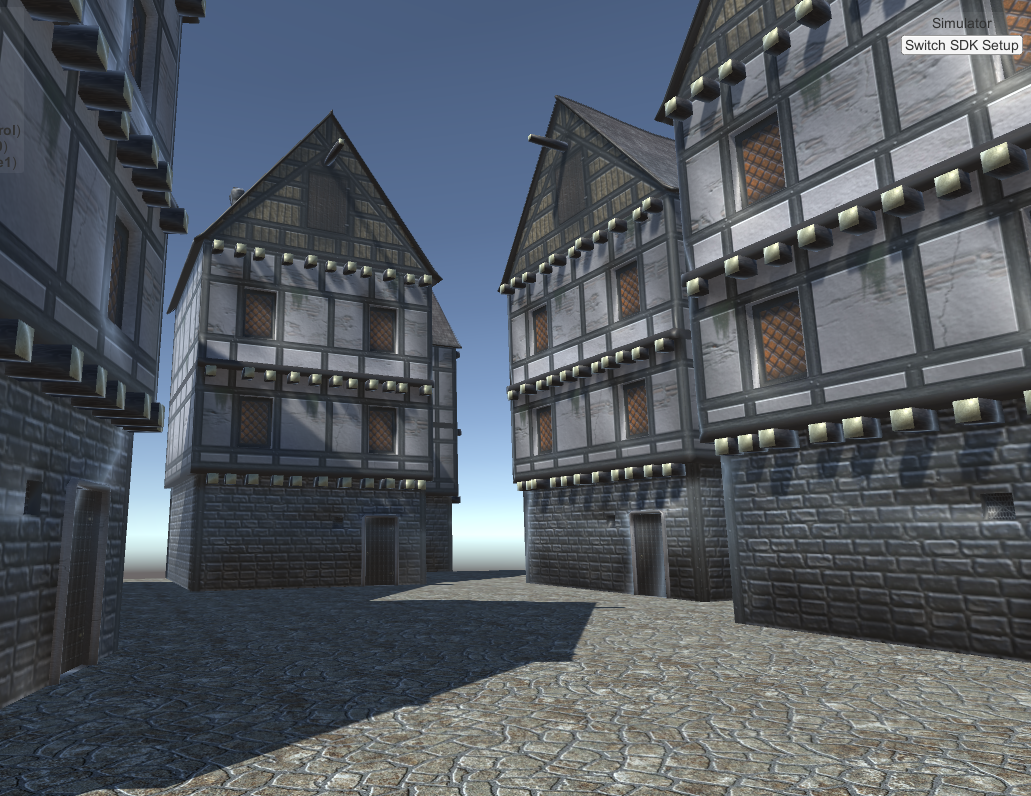
\includegraphics[width=\textwidth,height=\textheight,keepaspectratio]{screen1.png}
  		\caption{Ukázka běhu aplikace, modely budov převaty z~\cite{building}}
  		\label{fig:buildings}
	\end{figure}
    
    
    \subsection{Textury}
    
    Odkaz na textury je nadefinovaný v~proměnné, jejíž obsah byl získán z~databáze přes API. Textury jsou načítány ze souboru ve FS, který je v~této proměnné uložen. Soubor je otevřen, načten do pole bajtů a následně je toto pole bajtů vloženo do speciály třídy Texture2D, kterou interně definuje Unity. Kód tohoto načítání je převzat z~\cite{unityFAQtext}, ukázka níže.

\begin{lstlisting}[frame=single]
  public static Texture2D LoadTexture(string filePath)
    {

        Texture2D tex = null;
        byte[] fileData;
        Debug.Log("filepath = " + filePath);

        if (File.Exists(filePath))
        {
            fileData = File.ReadAllBytes(filePath);
            tex = new Texture2D(2, 2);
            tex.LoadImage(fileData);
        }
        return tex;
    }
        \end{lstlisting}	
        
        
    \subsection{StreamingAssets}
Tento prototyp načítá modely i textury za pomoci odkazu do FS, který získá přes API. Je pravděpodobné, že v~budoucnu bude naimplementováno i řešení, které si bude uchovávat binární soubory textur a 3D modelů přímo v~databázi, ovšem pro tuto bakalářskou práci bylo prozatím zvoleno toto řešení, neboť je praktičtější na testování a zároveň efektivnější z~hlediska fungování databáze.

To ovšem znamená, že i hotová zkompilovaná aplikace musí mít tyto odkazy na textury a modely k~dispozici. To by mohlo způsobovat problémy z~hlediska odkazů do FS, které by ve finálním nasazení aplikace už nemusely být na stejném místě, na kterém byly při vývoji.

Tento problém řeší Unity za pomocí složky StreamingAssets. Jedná se o~složku umístěnou v~adresáři Assets, ke které je možno přistupovat dynamicky. Pokud budou tedy všechny soubory, které aplikace za běhu dynamicky načítá, uloženy v~této složce, budou k~dispozici bez problémů i po kompilaci, neboť složka StreamingAssets je vždy nově vytvořena a přenesena i při kompilaci aplikace do nového projektu vedle spustitelného souboru. Ukázka dynamického volání souborů z~této složky a jejich následné využití je k~vidění níže:

\begin{lstlisting}[frame=single]
objPath = Path.Combine(Application.streamingAssetsPath, model.file_link);
texturePath = Path.Combine(Application.streamingAssetsPath, model.texture_link);

GetComponent<MeshFilter>().mesh = FastObjImporter.Instance.ImportFile(objPath);
Renderer rend = GetComponent<Renderer>();
rend.material.mainTexture = LoadTexture(texturePath);
\end{lstlisting}


	\section{Průběžná integrace}
	Průběžná integracie neboli continuous integration (CI), je proces, který zjednodušuje vývoj nového softwaru. Jedná se o proces, kdy se při každé změně přidané do repozitáře automaticky spustí kompilace celé aplikace na vzdáleném serveru. Díky tomu se jednak ušetří čas, jednak se zamezí mnohým chybám, které by mohly vzniknout, pokud by se celý (často dlouhý a komplikovaný) proces kompilace prováděl manuálně.
	
	\subsection{TravisCI}
Pro potřeby průběžné integrace této bakalářské práce byla zvolena technologie TravisCI. Jedná se o webovou službu propojenou s GitHubem. Pokud tedy vývojář používá GitHub, při každém spuštění příkazu \uv{git push} se automaticky spustí kompilace na systému TravisCI. K tomu je potřeba mít v hlavním adresáři gitového repozitáře konfigurační soubor \emph{.travis.yml} a také složku s názvem Scripts, která obsahuje ty skripty, které budou na serveru spuštěny (typicky tedy instalaci potřebných aplikací, kompilační skripty a testovací skripty). Výhoda průběžné integrace je nejen automatizace, ale také přehled o kompilaci na dálku, neboť při každém běhu služby TravisCI se výsledek přepošle vlastníkovi daného repozitáře na email.

\subsection{CI a Unity}
Pro potřeby průběžné integrace programů vyvíjených pod Unity 3D je potřeba na vzdálený server Unity nainstalovat. Toto zajistí skript install.sh, který stáhne potřebnou distribuci Unity a nainstaluje ji na vzdálený server. Poté je spuštěn soubor build.sh, který zkompiluje projekt z repozitáře pro všechny platformy, které jsou v tomto skriptu nadefinovány. Ukázka instalačního kódu převzatého pro tento účel z \cite{travis} je k vidění níže:

\begin{lstlisting}[frame=single]
#! /bin/sh

BASE_URL="https://download.unity3d.com/download_unity"
VERSION=2017.4.0f1

download() {
  file=$1
  url="$BASE_URL/52d9cb89b362/MacEditorInstaller/Unity-2017.4.2f2.pkg"

  echo "Downloading from $url: "
  curl -o `basename "$package"` "$url"
}

install() {
  package=$1
  download "$package"

  echo "Installing "`basename "$package"`
  sudo installer -dumplog -package `basename "$package"` -target /
}

install "MacEditorInstaller/Unity-$VERSION.pkg"
\end{lstlisting}

	\section{Grafické uživatelské rozhraní}
	\label{sec:GUI}
	
	Tato kapitola se bude věnovat všem náležitostem, které jsou spojeny s~tvorbou GUI. V~první části budou rozebrány specifika GUI pro technologie VR, v~druhé pak samotné návrhy GUI pro aplikaci Virtuální průvodce.
	
	
	\subsection{Použitelnost GUI pro VR}
VR headset je velice odlišné prostředí, než na jaké je většina uživatelů z~osobních počítačů či mobilních telefonů zvyklá. Navíc vzhledem k~dosavadním cenám VR ještě nejsou tyto technologie tak rozšířené, takže se s~nimi uživatelé setkávají spíše nahodile na různých akcích, ve VR hernách apod. Proto je nutné předpokládat, že uživatel, který naši aplikaci spustil, nikdy předtím VR headset na hlavě neměl. Tomuto předpokladu se musí návrh uživatelského prostředí podřídit a být tak jednoduchý a intuitivní, jak je to jen možné. Zcela jednoznačně bude dáván klad na minimalismus a přehlednost.
	
	\subsection{Prvotní návrh}
V~teté kapitole budou rozebrány prvotní návrhy (neboli wireframy) grafického uživatelského rozhraní. Finální verze se může nakonec lišit podle výsledků uživatelských testů.

	\subsubsection{Celkový koncept}
V~rámci GUI bývá v~dnešní době standardní základní menu obrazovka, která se skládá z~několika rovin, které uživatel vidí rozmístěné kolem sebe. Do této obrazovky je možné se vracet stiskem příslušného tlačítka na VR ovladačích. Je to první obrazovka, kterou uživatelé při spuštění uvidí, a zároveň se k~ní mohou vrátit kdykoli během samotného běhu aplikace. Otáčením hlavy dokola se pak uživatel rozhlíží po jednotlivých obrazovkách a interaguje s~nimi za použití ovladačů. Stejný přístup byl zvolen i pro tuto aplikaci. 

	\subsubsection{Výběr lokality}
Na této obrazovce si uživatel může zvolit, kde ve městě se chce v~danou chvíli nacházet. Na levé polovině mohou uživatelé buď vybírat libovolné body na mapě, nebo si v~levé polovině mohou vybrat konkrétní ulici ve městě z~nabídky.  Svůj výběr pak potvrdí tlačítkem OK, které je umístěné uprostřed pod oběma možnostmi výběru. Viz obr. \ref{fig:mockMisto}.

	\begin{figure}
  		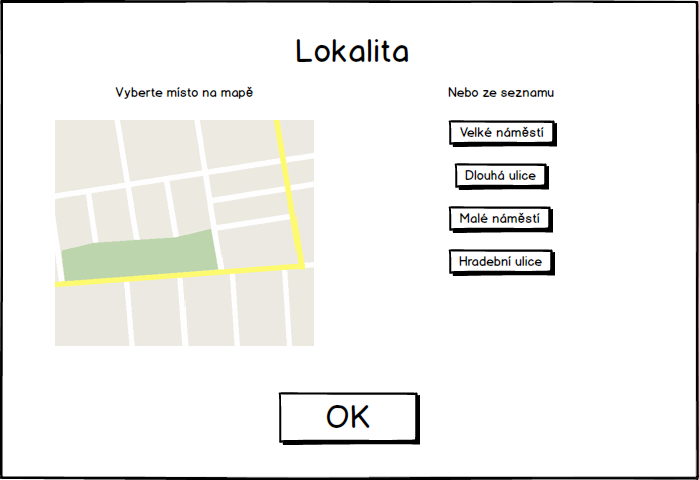
\includegraphics[width=\textwidth,height=\textheight,keepaspectratio]{MockMisto.png}
  		\caption{Wireframe pro vybírání místa}
  		\label{fig:mockMisto}
	\end{figure}
	
	\subsubsection{Výběr počasí}
Druhá obrazovka, která bude umístěna v~hlavním menu, bude výběr počasí. Zde si uživatelé mohou vybrat roční období, denní dobu a počasí v~dané scéně. Pro jednoduchost bude vždy jedna možnost předem vybraná, aby uživatelé nebyli nuceni proklikávat všechny varianty, i když chtějí změnit například jednu jedinou. Výběr potvrdí rovněž tlačítkem OK umístěným ve spodní části obrazovky. Viz obr. \ref{fig:mockPocasi}.
	
	\begin{figure}
  		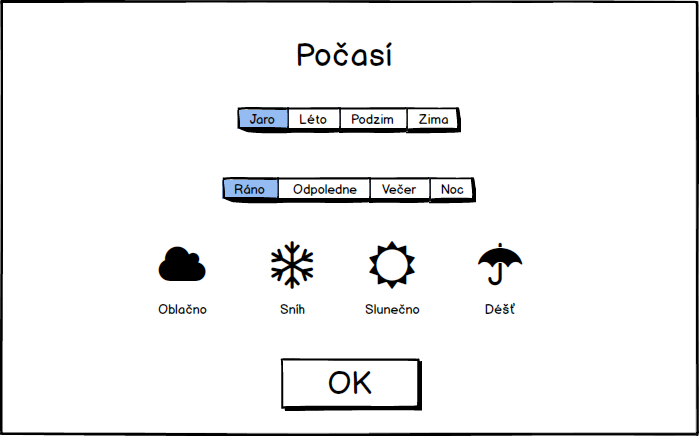
\includegraphics[width=\textwidth,height=\textheight,keepaspectratio]{MockPocasi.png}
  		\caption{Wireframe pro vybírání počasí}
  		\label{fig:mockPocasi}
	\end{figure}
	
	\subsubsection{Administrátorský režim}
Administrátorský režim, neboli režim architekta (Architect Mode), bude umožňovat vkládání nových budov, případně úprava budov stávajících. Předpokládáme, že tento mód bude využíván pouze v~PC verzi aplikace, protože je potřeba mít přístup a FS (pro vybrání souboru nově vkládané budovy) a ke klávesnici (pro vložení jejího popisu). Proto se při návrhu tohoto UI nemusí brát v~potaz specifika návrhu pro VR headset, wireframe na obr. \ref{fig:ArchitectMock} tudíž připomíná více klasické desktopové aplikace.

\begin{figure}
  		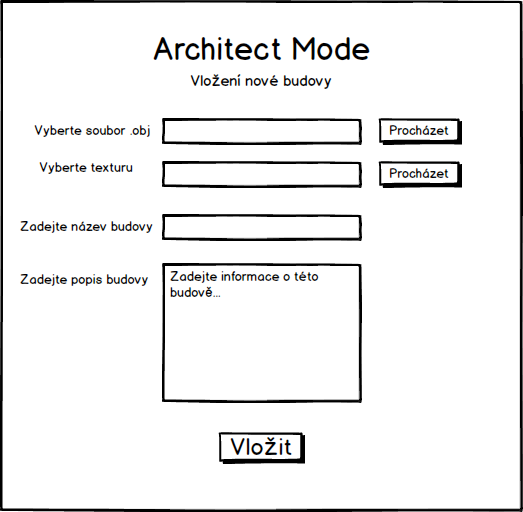
\includegraphics[width=\textwidth,height=\textheight,keepaspectratio]{ArchitectMock.png}
  		\caption{Wireframe pro režim architekta}
  		\label{fig:ArchitectMock}
	\end{figure}
	
	\section{Uživatelské testování}
	
	Testování nových aplikací uživateli samotnými před finálním nasazením je jedna z~nejdůležitějších částí vývoje kteréhokoli softwaru. Pro VR aplikace toto tvrzení platí o~to více, neboť se jedná o~velice nové technologie a tak ještě nejsou ustálené formy a ty stávající nejsou plně prověřeny časem.
	
	 Uživatelské testování přináší unikátní pohled cílové skupiny na daný software, který samotné vývojáře často dokáže překvapit. I~když je aplikace vyvíjena se znalostí nejdůležitějších principů UCD (user centred design), nikdy není jisté, že je pro uživatele přijatelná, dokud tak uživatelé sami neřeknou. Proto jsou data získaná formou uživatelského testování velice cennou informací pro tvorbu uživatelského rozhraní a často i logiky celého systému.
	
	\subsection{Specifika testování VR aplikací}
	
	Jak bylo zmíněno výše, VR brýle jsou zatím velice nové a časem neprověřené technologie, a o~to více je důležité aplikace pro ně vyvíjené náležitě otestovat. Tyto testy se v~určitých ohledech liší od klasického uživatelského testování pro mobilní či desktopové aplikace a to hned v~několika bodech.
	
	 Jako u~každého uživatelského testování je podstatné správně odhadnout svou cílovou skupinu a tedy i své testery. Proto bude do dotazníku k~uživatelskému testování (příloha \ref{sec:dotaznik}) na prvním místě položena otázka o~zkušenosti testerů s~VR zařízeními. Je rozdílné, když aplikaci používá někdo, kdo VR nikdy nepoužíval a někdo, kdo má vlastní VR headset doma.
	 
	 Dále bude podstatné zajistit dobrý prostor a seznámit se s~ním ještě před začátkem testování, neboť aplikace pro VR jsou téměř vždy používány v~prostoru a nejinak tomu bude i u~aplikace Virtuální historický průvodce.
	 
	 A~poslední, ovšem neméně podstatnou odlišností testování VR, je pohodlí uživatelů. Jakmile si tester nasadí VR brýle, tak najednou přijde o~jeden z~nejzákladnějších lidských smyslů, o~zrak. V~tu chvíli je nutné, aby se mu plně věnoval moderátor, tedy aby se ujistil, že brýle dobře sedí, aby uživatele naváděl v~prostoru a kontroloval, že zůstává ve vymezeném prostoru atd. Speciálně u~nových uživatelů VR může v~prvním okamžiku docházet k~pocitům nejistoty, nevolnosti či závratě, a proto je naprosto nezbytné, aby se moderátor postaral o~jejich pohodlí. \cite{VRuse}
	
	\subsection{Průběh testování aplikace}
	
	Testování aplikace Virtuální Historický průvodce proběhne v~rámci akce Muzejní noc 2018. Tato akce se bude konat až v~červnu letošního roku, proto budou výsledky testování známy později. Uživatelé budou vedeni aplikací za pomoci moderátora, který bude postupovat podle přiloženého scénáře (příloha \ref{sec:scenar}). Po vyzkoušení aplikace uživatelé vyplní dotazník (příloha \ref{sec:dotaznik}) ohledně použitelnosti aplikace.

	\section{Uživatelská příručka}
	
	V~této sekci budou popsány základní principy fungování aplikace Virtuální historický průvodce, včetně instalace a ovládání tohoto softwaru. Přestože výsledná aplikace bude přenositelná na různé VR zařízení, základní prototyp byl vyvíjen převážně pro stolní PC. Proto se zde věnujeme převážně instalaci a spuštění na PC.

\subsection{Instalace na PC}	
	Pokud aplikaci získáme ve formě souboru .zip, pak stačí tento soubor rozbalit do libovolného adresáře. Aplikace se sama nainstaluje a spustí poklepáním na soubor pruvodce.exe.
	
\subsection{Ovládání simulátoru}
Pokud aplikace není spuštěna přes VR headset, ale na stolním PC, je možné ji ovládat za pomocí simulátoru.\cite{VRTK} Následuje seznam základních ovládacích prvků tohoto simulátoru. Všechny klávesové zkratky jsou také popsány v~levém horním rohu aplikace samotné (obr. \ref{fig:simulator}).

\subsubsection{Mód ovládání kamery}
V~tomto módu uživatel automaticky začíná. Je možné se v~něm rozhlížet po okolí (ovládat pohled kamery simulující pohyby hlavy), ovšem není možné ovládat pohyby rukou. Klávesou levý Alt se pak může přepnout do módu ovládání pohybu rukou a zpět.


\begin{description}

	\item \textbf{Otáčení hlavy}
	
	Pohybem myši. 
	
	\item \textbf{Dálkový ukazatel}
	
	Tlačítko Q.		
	
	\item \textbf{Interakce}
	
	Tlačítka myši.
	
	
	\item \textbf{Chůze}
	
	Tlačítky W, A, S, D.	
	
	
	\item \textbf{Rychlá chůze}
	
	Levý Shift.
	
	\item \textbf{Hlavní menu}
	
	Tlačítko F.
	
\end{description}

\subsubsection{Mód pohybů rukou}
Simulátor zobrazuje ovladače v~rukou uživatele jako červený a zelený bod, které jsou ve výchozím nastavení umístěny pod hlavní kamerou (z~lidské anatomie pod úrovní hlavy), proto je dobré před prvním přepnutí do tohoto módu sklopit pohled kamery dolů. Přepínání mezi tímto módem a ovládáním kamery lze docílit stiskem klávesy levý Alt. Pro ilustraci viz obr. \ref{fig:simulator}.

\begin{description}

	\item \textbf{Pohyb rukou}
	
	\begin{itemize}
		\item V~osách x/z pohybem myši
		\item V~ose y stiskem Ctrl a následným pohybem myši
	\end{itemize}

	\item \textbf{Změna ovládané ruky}
	
	Stisknutím klávesy levý Tab.	

\end{description}

\begin{figure}
  		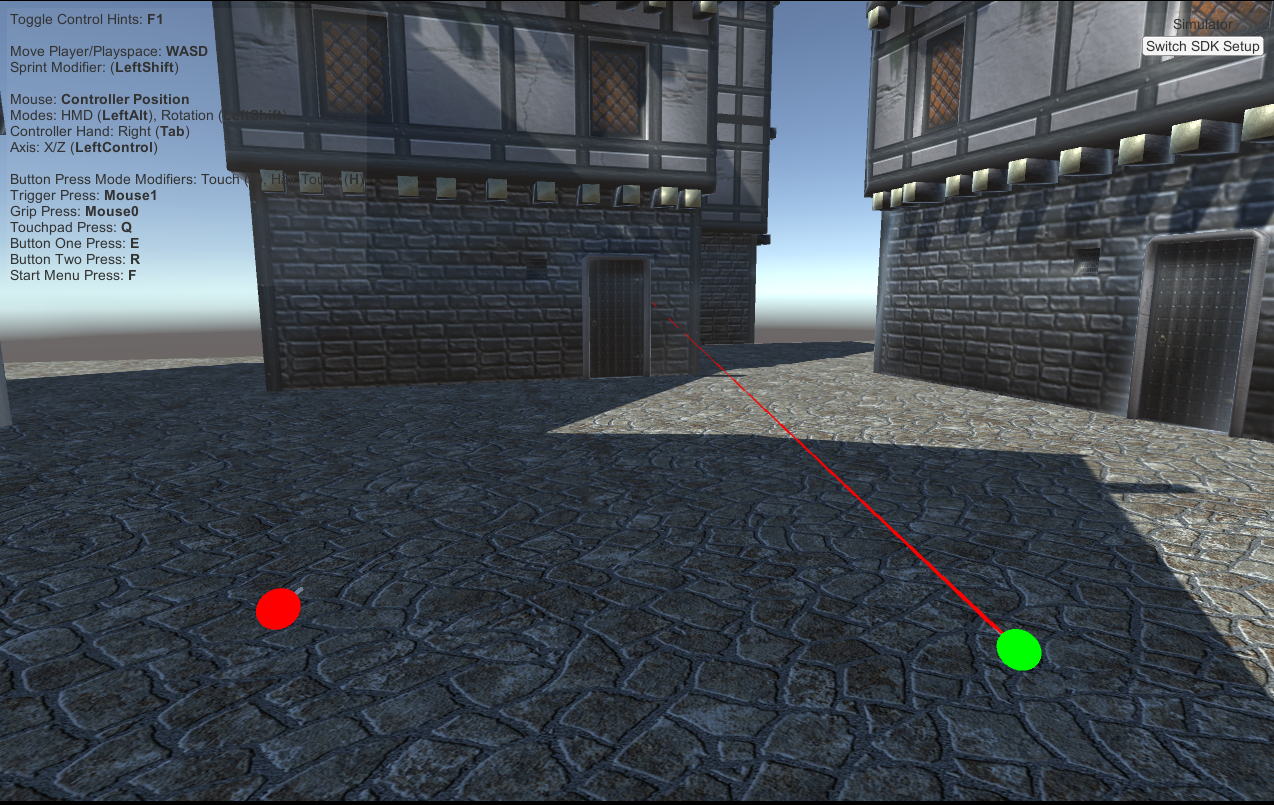
\includegraphics[width=\textwidth,height=\textheight,keepaspectratio]{screen2.png}
  		\caption{Ovládání simulátoru}
  		\label{fig:simulator}
	\end{figure}




\begin{conclusion}
	   
    Tato práce se zabývala vizualizací městské scenérie a je součástí týmového projektu Virtuální Historický Průvodce. Jejím výstupem byla aplikace, která umožňuje uživatelům prozkoumávat středověká města za pomocí technologií virtuální reality. Jedná se o~řešení, které ukládá  logickou strukturu města v~databázi a díky tomu pak zobrazuje pouze ty budovy, které se nacházejí k~uživateli nejblíže, čímž se jednoznačně zvýší její efektivita. Uživatel výsledné aplikace bude s~její pomocí přenesen na konkrétní lokaci v~daném městě a kolem něj budou vygenerovány nejbližší domy s~ohledem na dané počasí a denní dobu.  Tohoto bylo úspěšně dosaženo, jak je možné zjistit z~přiložených zdrojových kódu a spustitelných souborů v~příloze.
    
     V~budoucnu bude tato aplikace sloužit jako prototyp pro robustnější systém, který mimo jiné umožní také podporu smíšené reality, nasazení na Android a další možnosti. Jedná se o~projekt, který chce oslovit kromě běžných uživatelů také odborníky z~pole humanitních věd, především historie, dějin umění, archivnictví a architektury. Díky jednoduchému a intuitivnímu uživatelskému rozhraní by tato aplikace mohla být nasazena i v~těchto oborech, kde může přispět k~vizualizaci starých měst. Došlo by tak k~rychlým a efektivním vědeckým pokrokům díky užší spolupráci mezi humanitními a technickými obory.
\end{conclusion}

\bibliographystyle{csn690}
\bibliography{mybibliographyfile}



\appendix

\chapter{Seznam použitých zkratek}
% \printglossaries
\begin{description}
	\item[2D] Two dimensional, dvojrozměrný
	\item[3D] Three dimensional, trojrozměrný
	\item[API] Apliaction programming interface,  rozhraní pro programování aplikací
	\item[AR] Augmented reality, rozšířená realita
	\item[CI] Continuous integration, průběžná integrace
	\item[CLR] Common Language Runtime, runtime pro C\#
    \item[CityGML] Aplikační schéma pro reprezentaci GML
	\item[COLLADA] Formát pro interaktivní 3D scény, XML schéma
	\item[DL] Datová Layer, datová vrstva
	\item[ER] Entitně vztahový model databáze
	\item[FS] File System, souborový systém
	\item[GML] Geography Markup Language, geografický značkovací jazyk
	\item[GUI] Graphical user interface, grafické uživatelské rozhraní
	\item[HMD] Head-mounted display, neboli headset, VR brýle
	\item[HK] Hradec Králové, projekt na téma vizualizace věnných měst
    \item[JRE] Java Runtime Environment, rozhraní pro Java aplikace
    \item[JSON] Javascriptový objektový zápis, běžný formát pro přenos dat
	\item[LoD] Level of Detail, úroveň detailu grafických modelů
	\item[KML] Keyhole Markup Language, XML vyvinuté pro google earth
    \item[.NET] Knihovna spojená s~jazykem C\#
    \item[NpSQL] Knihovna pro navázání spojení s~databází v~.NET
    \item[.OBJ] Frekventovaný formát 3D
    \item[PostgreSQL] Open source RDBMS
    \item[PostGIS] Geografický PostgreSQL
	\item[REST] Representational state transfer, architektura rozhraní
	\item[RDBMS] Systém pro správu relačních databází
	\item[SDK] Software development kit, sada vývojových nástrojů 
	\item[SP2] Softwarový týmový projekt 2, předmět na FIT ČVUT
	\item[VR] Virtual reality, virtuální realita
    \item[WebGL] Javascriptové API pro zobrazování 3D grafiky
    \item[UI] Uživatelské rozhraní
    \item[UCD] User Centred Design, návrh z~hlediska uživatele
    \item[VRML] Formát pro popis 3D scén a virtuální reality
    \item[VRTK] Sada skriptů pro vývoj VR aplikací v~Unity 3D
	\item[XML] Extensible markup language, rozšiřitelný značkovací jazyk
	\item[XR] Zastřešující pojem pro technologie virtuální, rozšířené a smíšené reality
	\item[YAML] Formát pro serializaci strukturovaných dat
\end{description}


\chapter{Obsah přiloženého USB}


\begin{figure}
	\dirtree{%
		.1 readme.txt\DTcomment{stručný popis obsahu USB}.
		.1 exe\DTcomment{adresář se spustitelnou formou implementace}.
		.1 src.
		.2 impl\DTcomment{zdrojové kódy implementace}.
		.2 thesis\DTcomment{zdrojová forma práce ve formátu \LaTeX{}}.
		.1 text\DTcomment{text práce}.
		.2 thesis.pdf\DTcomment{text práce ve formátu PDF}.
		.2 thesis.ps\DTcomment{text práce ve formátu PS}.
	}
\end{figure}

\chapter{Scénář uživatelského testování} \label{sec:scenar}
Přiložený scénář testování bude použit při prvním zkušebním nasazení aplikace, které by mělo proběhnout na pražské muzejní noci 2018. Tento scénář je provázen dotazníkem, který je taktéž k~vidění v~příloze \ref{sec:dotaznik}.
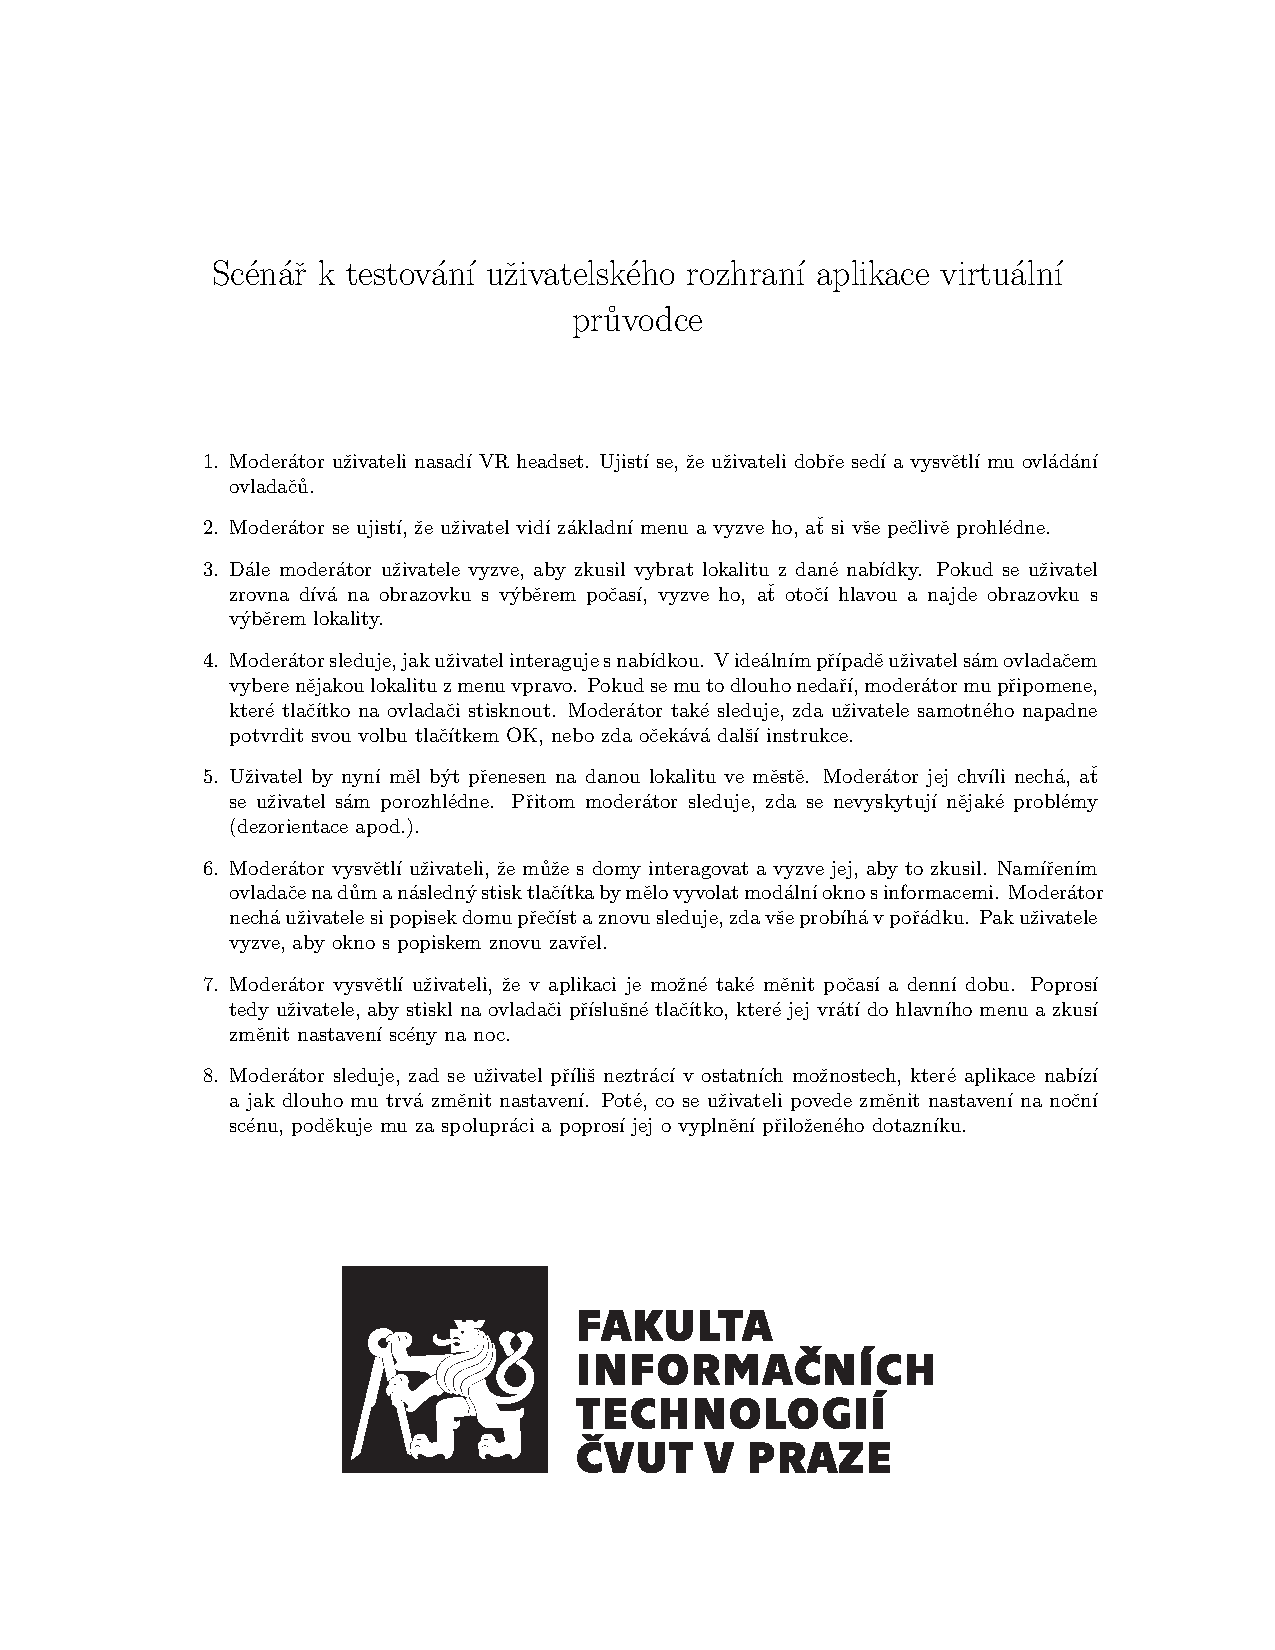
\includepdf[pages={1}]{scenar.pdf}
\chapter{Dotazník pro uživatelské testování} \label{sec:dotaznik}
Tento dotazník bude nasazen při uživatelském testování aplikace. Uživatelé jej vyplní poté, co si aplikaci vyzkouší podle scénáře, který je taktéž přiložen k~této práci v~příloze \ref{sec:scenar}.
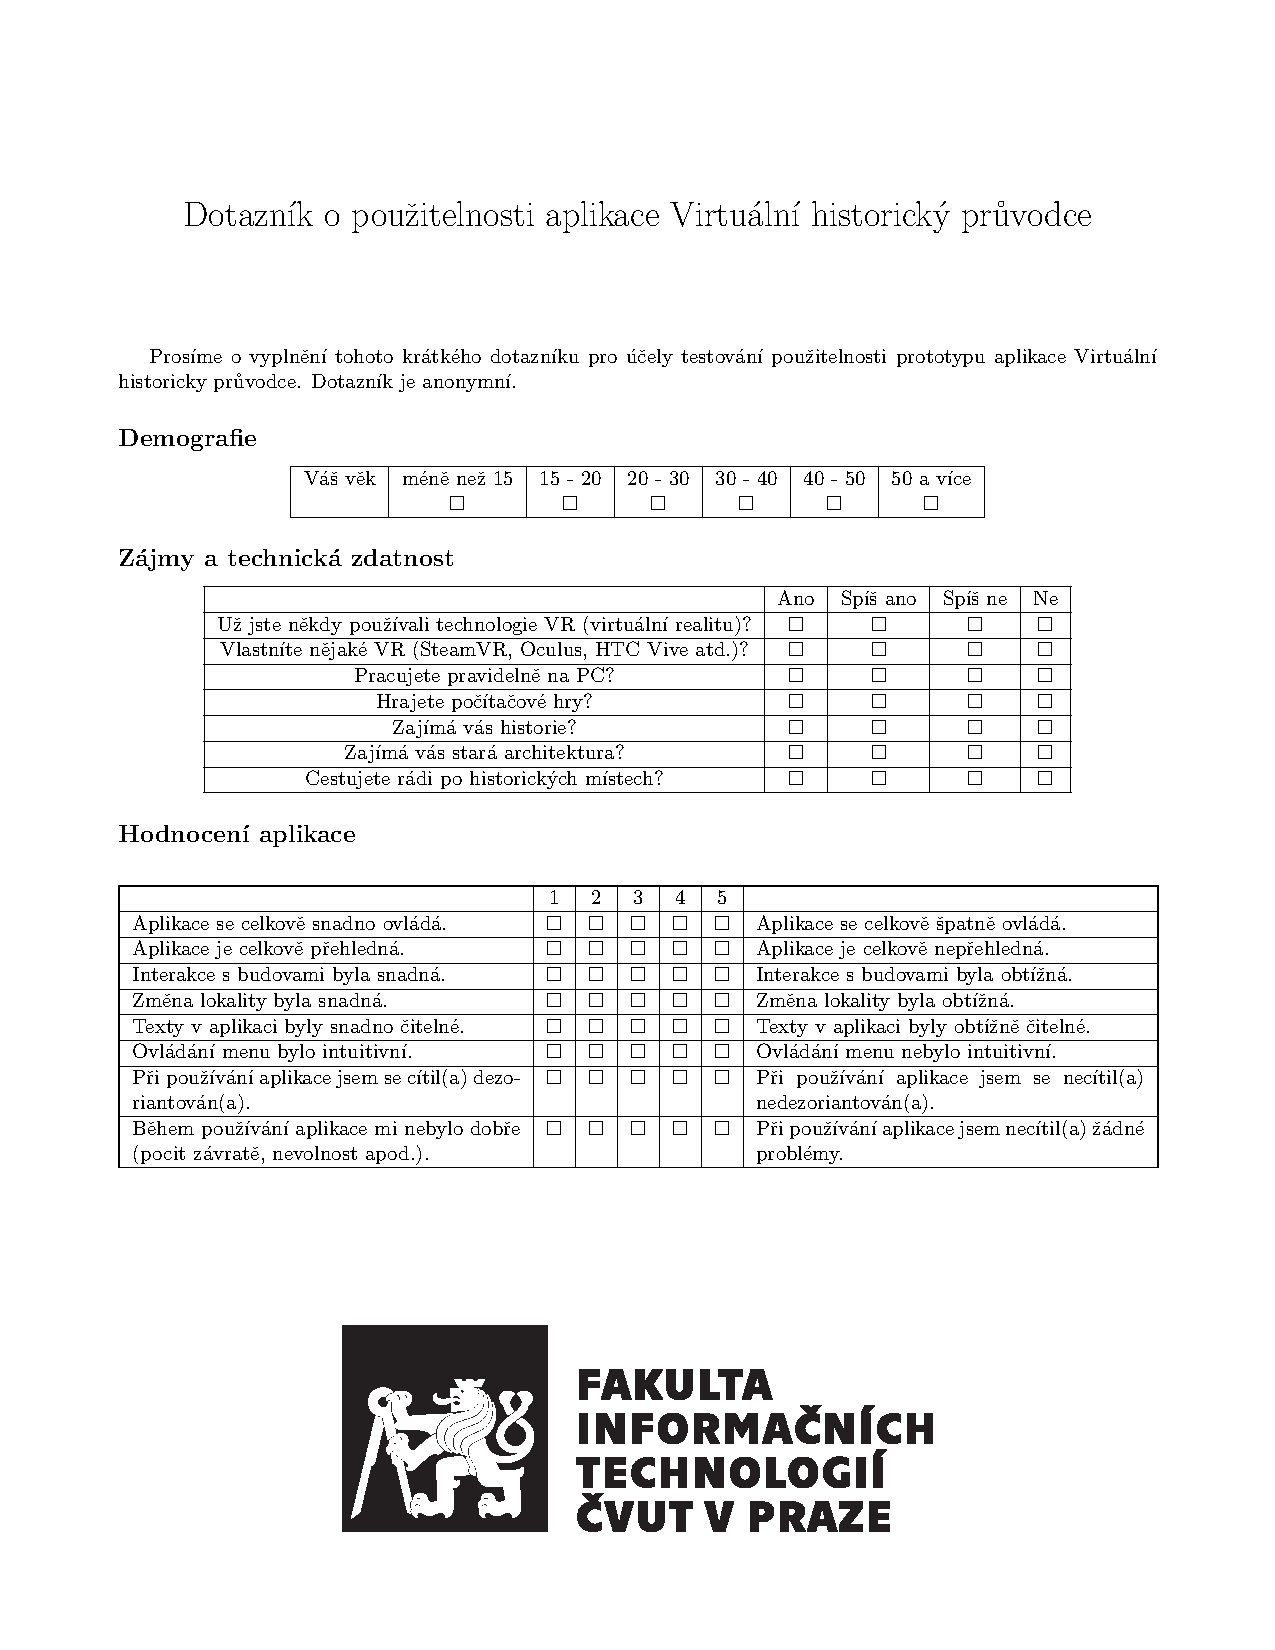
\includepdf[pages={1}]{dotaznik.pdf}

  

\end{document}
